\documentclass[12pt]{article}
\usepackage[margin=1in]{geometry}
\usepackage{setspace}
\usepackage{amsmath,amssymb,amsthm}
\usepackage{graphicx}
\usepackage{booktabs}
\usepackage{multirow}
\usepackage{array}
\usepackage{algorithm}
\usepackage{algorithmic}
\usepackage{xcolor}
\usepackage[round,authoryear]{natbib}
\let\cite\citep
\usepackage{url}
\usepackage{textcomp}
\usepackage[hidelinks]{hyperref}
\newtheorem{definition}{Definition}
\newtheorem{proposition}{Proposition}
\newtheorem{theorem}{Theorem}
\newtheorem{corollary}{Corollary}
\newtheorem{finding}{Finding}
\begin{document}
\onehalfspacing
\title{Context-Augmented, Session-Calibrated Blood Pressure Tracking from Photoplethysmography}
\author{Farouk Ganiyu Adewumi and Timothy Oladunni\\
\normalsize Department of Computer Science, Morgan State University, Baltimore, MD 21251, USA\\
\normalsize \texttt{fagan1@morgan.edu}; \texttt{timothy.oladunni@morgan.edu}}
\date{}
\maketitle
\begin{abstract}
\textbf{Objective.} To determine whether acquisition context and photoplethysmography (PPG) features improve session-calibrated blood pressure tracking while controlling participant leakage and calibration burden.

\textbf{Approach.} We performed repeated five-fold participant-level cross-validation on 653 AuroraBP participants, excluding calibration-labelled rows from fitting and scoring. We also conducted a feature-family ablation, an independent 108-participant pulse-rate fusion analysis, and a separately developed VitalDB evaluation on 227 held-out subjects.

\textbf{Main results.} With a three-reading cuff anchor, the wearable-state model achieved participant-level mean absolute errors of $7.697$~mmHg for systolic blood pressure (SBP) and $6.139$~mmHg for diastolic blood pressure (DBP). Wearable context reduced error by $0.436$~mmHg for SBP (97.5\% confidence interval $0.305$--$0.573$) and $0.126$~mmHg for DBP ($0.053$--$0.200$). Standard PPG descriptors provided further reductions of $0.187$~mmHg for SBP and $0.180$~mmHg for DBP, whereas nonlinear/attractor features did not show a reliable benefit. Quality-weighted visible/infrared fusion reduced pulse-rate error from $3.985$ to $3.690$~beats per minute. In VitalDB, combining context and PPG predictions reduced error by $0.451$~mmHg for SBP and $0.357$~mmHg for DBP, although absolute error remained $15.375$ and $8.833$~mmHg, respectively.

\textbf{Significance.} Context and standard PPG descriptors produced reproducible but clinically small improvements. The results support calibrated tracking research but do not establish model transfer, equitable performance, standards compliance, or cuff replacement.
\end{abstract}
\noindent\textbf{Keywords:} photoplethysmography; cuffless blood pressure; session calibration; participant-level cross-validation; wearable sensing; data leakage; signal quality.
\section{Introduction}
\label{sec:intro}
\subsection{Motivation}
PPG-based cuffless BP estimation is attractive because optical sensors are already present in consumer wearables. Its evaluation must distinguish participant overlap, calibration burden, and acquisition-context shortcuts. Record-level splits can inflate apparent accuracy when correlated measurements from one participant enter both training and testing \cite{bpbenchmark2023}. A model anchored to three initial cuff readings also answers a different question from one calibrated once or repeatedly supplied with recent cuff values. Finally, pigmentation-associated optical differences motivate intervention testing, but a small subgroup or a nonsignificant contrast cannot establish equitable performance \cite{fitzpatrick2024,jmir2024,phantom2026}.
We audit anchoring, context, and pigmentation-related interventions using recorded Fitzpatrick labels. Candidate interventions and context arms were frozen before repeated participant-level validation, after earlier development on AuroraBP. Because a fixed holdout was inspected across successive ablations, it is retained as historical development evidence. The primary repeated analysis confines feature ranking and fitting to outer training participants but remains internal validation. Secondary negative results are reported without interpreting them as proof of equity, equivalence, or general failure of pigmentation-aware modeling.
\subsection{Study Questions and Contributions}
The primary question is whether wearable-state context improves session-anchored SBP and DBP tracking beyond the same calibrated model core. Secondary analyses test calibration dose, standard versus nonlinear/attractor PPG feature families, and pigmentation-related interventions. Historical development analyses examine how recent-cuff anchoring can inflate apparent gains. These questions were specified retrospectively; repeated cross-validation estimates internal stability rather than prospective confirmation.

The study contributes participant-separated evaluation of wearable context, a calibration-row leakage audit, and matched calibration-dose and feature-family comparisons. Independent analyses evaluate visible/infrared pulse-rate fusion and a separately developed VitalDB context-plus-PPG model. Negative pigmentation-intervention and attractor-ablation findings are retained without claims of equity or physiological validation. Historical development results and auxiliary diagnostics appear in the supplementary material.
\section{Related Work}
\label{sec:related}
\subsection{PPG-Based Cuffless Blood Pressure Estimation}
Cuffless BP estimation from PPG includes pulse-transit-time methods, waveform features, and end-to-end networks \cite{elgendi2019ppg,mukkamala2015toward}. Calibration-free methods avoid subject-specific references, whereas calibrated approaches use one or more cuff readings to model subsequent change \cite{calfree2023,onetimecal2023,avct2026}. Evaluation guidance emphasizes participant separation, calibration burden, and careful use of AAMI/ISO~81060-2 and BHS criteria \cite{recommendations2024}.
\subsection{Nonlinear and Information-Theoretic Feature Representations}
The feature bank combines waveform moments with delay-coordinate reconstruction, recurrence analysis, sample entropy, permutation entropy, and spectral measures \cite{takens1981,eckmann1987,marwan2007,richman2000,bandt2002}. These established descriptors have been applied to physiological and arterial pulse signals \cite{allen2007ppg,attractorpulse2022}. Recent author-developed formulations motivated the feature grouping and terminology \cite{cst2026,avct2026,adt2026}, but are not treated as validated physiological laws. The matched ablation therefore tests the empirical contribution of the combined nonlinear/attractor family rather than using prediction as evidence for the underlying theories.
\subsection{Skin Pigmentation and PPG-Derived Vitals}
Pigmentation can affect optical measurements, motivating separate evaluation of signal quality and downstream error \cite{jmir2024,fitzpatrick2024,phantom2026,montecarlo2026}. Existing field, polarization, and gain-correction studies support testing optical interventions but do not establish improved BP tracking \cite{equity2026,polarimetric2026,gaincorrection2025}. We therefore distinguish pulse extraction from BP prediction and do not interpret nonsignificant subgroup differences as parity.
\subsection{Evaluation Rigor and Data Leakage}
AuroraBP established calibration-based benchmarks and documented differences between laboratory and ambulatory performance \cite{aurorabp2022}. Record- or window-level splits can inflate reported accuracy when one participant contributes to training and testing \cite{bpbenchmark2023,mimicbp2024}, while dataset shortcuts may further obscure the information contributed by PPG \cite{limitations2024,challenges2024}. Our audit addresses a related change-prediction artifact: a calibration-row indicator may reveal observations whose target is near zero even when participant folds are disjoint.
\section{Framework and Audit Controls}
\label{sec:framework}
\subsection{Attractor Feature Bank}
Let $x_n$, $n = 1,\dots,T$, denote a discretely sampled PPG window at rate $f_s$. Following delay-coordinate embedding \cite{takens1981}, we reconstruct the trajectory
\begin{equation}
\mathbf{X} = \tau_{\mathcal{G}}[x], \qquad \mathbf{X}_{n,\cdot} = [x_n, x_{n+\tau}, \dots, x_{n+(d-1)\tau}],
\label{eq:embed}
\end{equation}
with embedding dimension $d = 4$ and delay $\tau = 5$ samples, matching the AVCT/CST instantiation \cite{avct2026,cst2026}. From $\mathbf{X}$ we compute the shared PPG attractor feature bank
\begin{equation}
\begin{aligned}
\Phi(x) = [\,&\sigma_m,\ \mathrm{skew}_m,\ \mathrm{kurt}_m,\ H_{\mathrm{SE}},\ H_{\mathrm{PE}},\ R_{\mathrm{rec}},\\
&R_{\mathrm{det}},\ H_{\mathrm{RQA}},\ \mathrm{CSI},\ H_{\mathrm{spec}},\ Q\,]
\end{aligned}
\label{eq:featurebank}
\end{equation}
comprising waveform moments ($\sigma_m$, skewness, kurtosis), sample and permutation entropy ($H_{\mathrm{SE}}$, $H_{\mathrm{PE}}$), recurrence rate and determinism ($R_{\mathrm{rec}}$, $R_{\mathrm{det}}$), recurrence entropy ($H_{\mathrm{RQA}}$), CSI, spectral entropy, and optical quality. The auxiliary stress-test bank labels the unmodified measured waveform \texttt{ref\_*}, the simulated stressed waveform \texttt{raw\_*}, and its corrected version \texttt{pc\_*}; ``reference'' does not mean latent physiological ground truth. AuroraBP instead extracts \texttt{raw\_*} from observed optical waveforms and \texttt{pc\_*} after the correction below. It does not construct an AuroraBP \texttt{ref\_*} input. The primary candidate pool contains raw-feature changes, time variables, and a UCI-derived prior; its exact provenance is described in Section~\ref{sec:features}.
\subsection{Pigmentation Correction Operator}
\label{sec:pcop}
The implemented AuroraBP operator is a heuristic motivated by attenuation, rather than an estimate of melanin or a fitted Beer--Lambert law. Let $z=(\mathrm{FST}-1)/5$, $b=\operatorname{median}(x)$, $a=\max(0.45,1-0.55z)$, and $u=(x-b)/a$. With $W(u)$ a Wiener-filtered version of $u$ and $\lambda=\operatorname{clip}(0.75z,0,0.75)$, the corrected channel is $b+(1-\lambda)u+\lambda W(u)$. The filter kernel is an odd number of samples derived from $0.05f_s$, bounded between 5 and 21. A residual-to-bandpassed-signal SD ratio, clipped to $[0,1.5]$, modifies entropy/recurrence tolerances; the corrected channel uses 0.35 times that ratio. The waveform median is a baseline proxy, not a separate measured DC channel. In the repeated participant-CV ablation, corrected-minus-raw MAE was $-0.007$~mmHg SBP (95\% CI $-0.042$ to $0.029$) and $-0.030$~mmHg DBP ($-0.062$ to $0.003$). These intervals do not establish overall benefit or equivalence. The ablation tests the complete correction-and-feature-extraction configuration, not attenuation rescaling alone.
\subsection{Calibration Dose and Anchoring}
\label{sec:anchoring}
For participant $p$, let $b_p^{(k)}$ denote an anchor formed from exactly $k$ initial cuff readings ($k\in\{1,2,3\}$), with $k>1$ using their arithmetic mean. We define the \emph{session-anchored} target
\begin{equation}
\Delta_{\mathrm{session}}^{(k)}(p,i) = y_{p,i} - b_p^{(k)},
\label{eq:sessionanchor}
\end{equation}
where $y_{p,i}$ is the $i$-th subsequent cuff reading for participant $p$, and the \emph{prior-anchored} target
\begin{equation}
\Delta_{\mathrm{prior}}(p,i) = y_{p,i} - y_{p,i-1}^{*},
\label{eq:prioranchor}
\end{equation}
where $y_{p,i-1}^{*}$ is the most recent valid prior measurement (which may itself be a tracked, non-calibration reading). \textbf{These are not the same question.} Eqn.~\ref{eq:sessionanchor} evaluates BP change after an initial calibration session without supplying later cuff values to the predictor. Eqn.~\ref{eq:prioranchor} asks whether PPG can track change from the most recent cuff reading, which in this in-lab protocol can be only minutes old. A model evaluated under Eqn.~\ref{eq:prioranchor} solves an easier problem; $83\%$ of the historical fixed-split gain under prior anchoring was attributable to anchor replacement alone. We therefore lead with session-anchored tracking results and explicitly report calibration dose; neither anchoring scheme establishes cuff replacement. ``One reading'' refers only to $k=1$; the primary $k=3$ analysis is described as \emph{one-session calibration using three readings}.
The \emph{calibration-retention baseline} predicts $\hat{\Delta} = 0$ under either anchor, i.e., ``the BP has not changed since calibration (or since the last reading).'' This is one baseline; the main context contrasts compare fitted models, and VitalDB additionally uses a calibration-plus-context control.
\subsection{Context Operator}
\label{sec:context}
Let $c(p,i)$ collect acquisition context. We distinguish a \emph{wearable-state} set (posture, activity, and optical signal quality) from a \emph{protocol-enriched} set that additionally includes protocol phase, recording duration, and pressure-quality metadata. The wearable-state variables require corresponding sensing or classification at deployment; the protocol-enriched variables may encode AuroraBP acquisition structure and are therefore interpreted as an internal upper bound on context utility. The context-augmented model is
\begin{equation}
\hat{\Delta}(p,i) = f_\theta\big(\Phi(x_{p,i}),\, \Phi(x_{p,i}) - \Phi(x_{p,\mathrm{anchor}}),\, c(p,i)\big),
\label{eq:model}
\end{equation}
where $f_\theta$ is a gradient-boosted tree ensemble (HistGradientBoosting; hyperparameters grid-searched over learning rate, maximum leaf nodes, and $\ell_2$ regularization) trained with either squared or absolute loss (Section~\ref{sec:methods}), and the first-difference term $\Phi(x_{p,i}) - \Phi(x_{p,\mathrm{anchor}})$ is the attractor-feature analogue of Eqns.~\ref{eq:sessionanchor}--\ref{eq:prioranchor} in feature space.
\subsection{Calibration-Row Leakage Audit}
\label{sec:leakage}
A calibration indicator could identify trivial rows if a target reading were compared with itself, allowing a model to learn ``calibration row $\Rightarrow$ predict no change.'' We used four checks:
\begin{itemize}
\item[\textbf{A}] Compare $|\Delta|$ on flagged and unflagged rows.
\item[\textbf{B}] Re-score the same fitted models with flagged rows removed from the holdout only.
\item[\textbf{C}] Refit with the calibration-flag feature removed, flagged rows still scored.
\item[\textbf{D}] \textbf{(Decisive)} Remove the flag and exclude flagged rows from fitting and scoring.
\end{itemize}
Checks A--C each leave one channel open; Check D restricts both fitting and evaluation. Supplementary Section B-F reports all four.
\begin{finding}
On this dataset, calibration-flagged rows are \emph{not} near-zero-delta (mean $|\Delta|=6.774$ vs.\ $9.902$~mmHg SBP on development rows -- smaller, but not trivially so), and Check D confirms the context gain survives essentially intact ($+0.614$ vs.\ the unaudited $+0.809$~mmHg SBP). Leave-one-out results implicate recording duration and post-exercise activity rather than the calibration flag (Supplementary Section B-F).
\end{finding}
\section{Methodology}
\label{sec:methods}
\subsection{Datasets}
\label{sec:datasets}
\textbf{AuroraBP} is the primary dataset \cite{aurorabp2022,aurorabpDataset}. It contains 1{,}221 participant records and 11{,}597 auscultatory measurements across calibration, static, exercise, and temporal-challenge phases; waveforms were resolvable for 672 participants. The primary common cohort includes 653 participants with three initial calibration readings. Excluding 1{,}337 later calibration-labelled rows leaves 7{,}879 scored measurements. Historical ablations used a fixed 501/168 split; because its holdout was inspected during development, it is treated as historical evidence rather than untouched validation.
Four secondary sources appear in the development notebooks: BIDMC, MIMIC-II, Welltory-PPG, and UCI \cite{bidmcDataset,pimentel2017,physionet2000,mimicii2011,mimiciiDataset,welltory2021,uciCufflessDataset,kachuee2015}. The first three form a historical corrected-feature PCA bank whose coordinates are excluded from the primary candidate list. UCI trains the BP-change prior that may enter the primary model. Pigmentation ranks on these sources are synthetic simulation inputs, not measured traits, and support no equity claim.

Two datasets support independent follow-up analyses. The \textbf{Appel--Theart Participant Study Data} provide paired visible and infrared PPG, Monk Skin Tone (MST), and pulse-rate references \cite{appel2025ppg}. After auditing, 108 participants contributed 630 pulse-rate windows, including 24 participants with MST~7--10. Its single cuff BP value per participant permits only cross-sectional BP analysis. \textbf{VitalDB} provides synchronized intraoperative PPG and arterial BP \cite{lee2022vitaldb,vitaldbDataset}. A locked evaluation used 5{,}472 future windows from 228 cases belonging to 227 subjects disjoint from the 55 development subjects. Cases were grouped by subject for inference. VitalDB has no skin-tone field and tests a separately developed intraoperative implementation, not transfer of AuroraBP-fitted parameters.
Table~\ref{tab:datasetsummary} consolidates the analysis sample, role, and source references for every dataset used in the study.
\begin{table*}[t]
\centering
\caption{Datasets Used}
\label{tab:datasetsummary}
\scriptsize
\renewcommand{\arraystretch}{1.12}
\begin{tabular}{>{\raggedright\arraybackslash}p{1.7cm}>{\raggedright\arraybackslash}p{3.0cm}>{\raggedright\arraybackslash}p{4.4cm}>{\raggedright\arraybackslash}p{5.2cm}}
\toprule
Dataset & Material analyzed & Role in this study & Source and access \\
\midrule
AuroraBP & 1{,}221 released participant records; 653 participants and 7{,}879 measurements in the strict primary endpoint & Primary session-calibrated BP evaluation, context arms, calibration dose, subgroup diagnostics, and feature-family ablation & Microsoft Research study and Zenodo dataset; available upon application under the provider's Data Use Agreement \cite{aurorabp2022,aurorabpDataset} \\
BIDMC & 53 subjects; 1{,}272 windows & Historical corrected-feature PCA representation; not a primary evaluation cohort & BIDMC PPG and Respiration Dataset, PhysioNet \cite{bidmcDataset,pimentel2017,physionet2000} \\
MIMIC-II & 1{,}500 sampled windows & Historical corrected-feature PCA representation; not a primary evaluation cohort & MIMIC-II Clinical Database, PhysioNet \cite{mimicii2011,mimiciiDataset,physionet2000} \\
Welltory-PPG & 106 windows & Historical corrected-feature PCA representation; not a primary evaluation cohort & Published PPG signal collection \cite{welltory2021} \\
UCI Cuff-Less BP & 425 records; 3{,}268 windows & Training source for the BP-change prior that may enter AuroraBP models & UCI Machine Learning Repository \cite{uciCufflessDataset,kachuee2015} \\
Appel--Theart & 108 analyzed participants; 630 pulse-rate windows & Independent visible/infrared quality-fusion and guarded MST-correction analysis & Mendeley Data \cite{appel2025ppg} \\
VitalDB & 55 development subjects; 228 held-out cases from 227 subjects; 5{,}472 scored future windows & Independent intraoperative calibration-plus-context and context-plus-PPG BP tracking & VitalDB and PhysioNet \cite{lee2022vitaldb,vitaldbDataset} \\
\bottomrule
\end{tabular}
\begin{minipage}{0.96\textwidth}
\vspace{2pt}\footnotesize Counts describe the material used by this study and need not equal the full source repository. Auxiliary-source pigmentation ranks were synthetic simulation inputs; only AuroraBP supplied Fitzpatrick labels and Appel--Theart supplied Monk Skin Tone labels.
\end{minipage}
\end{table*}
\subsection{Feature Extraction and Selection}
\label{sec:features}
AuroraBP features are extracted from the central 10-s optical window at $f_s=500$~Hz (5{,}000 samples), using a third-order 0.5--8~Hz bandpass, $d=4$, and $\tau=5$ samples (10~ms). The extractor calculates $f_s=(N-1)/(t_{N-1}-t_0)$ from the recording timestamps; all 11{,}427 cached feature rows match the timestamp audit at 500~Hz within $2\times10^{-11}$~Hz. The central waveform is not resampled before filtering. Sample entropy uses order 2, a base standardized tolerance of 0.2, and at most 600 samples; permutation entropy uses order 3. Recurrence analysis uses at most 300 standardized embedded points, Chebyshev distance, a base radius of 0.2 modified by the noise ratio, and diagonal lines of length at least 2. For the filtered AuroraBP signal, let $S(f)$ be its Welch power spectral density, with 4-s Hann segments and 50\% overlap. The quality feature is
\begin{equation}
Q=\frac{\sum_{0.5\le f\le5}S(f)}{\sum_{0.1\le f\le15}S(f)}.
\label{eq:auroraquality}
\end{equation}
CSI is $0.4R_{\mathrm{det}}+0.3[1-\operatorname{clip}(H_{\mathrm{RQA}}/5,0,1)]+0.3Q$. Recalculation from the cached components agrees with stored CSI to $2.3\times10^{-16}$. This derived spectral ratio, stored as \texttt{raw\_ppg\_quality}, is distinct from AuroraBP's supplied \texttt{optical\_quality} context field and the independent pulse-fusion weights $q_V,q_I$. The historical hybrid calibration-anchored feature augmentation is denoted HCA below; its source-code identifiers retain the older name H1, distinct from hypothesis H1.

Within each outer training fold, the primary code ranks raw-feature differences and relative differences, elapsed-time variables, and the UCI prior after ridge residualization against baseline BP and log elapsed time. It applies \texttt{mutual\_info\_regression} to the residuals and retains up to 24 candidates plus baseline BP. SMD and AUC were historical diagnostics, not the primary selection algorithm. The name ``no context'' means no \emph{added} context variables: baseline BP, candidate elapsed-time terms, and the UCI prior can still enter its shared core. No \texttt{ref\_*} feature enters that core. The UCI prior is generated from corrected features, so absence of explicit Fitzpatrick terms does not prove absence of indirect Fitzpatrick dependence. The regenerated selection manifests retain the UCI prior in 26 of 30 endpoint/fold core models; all context arms share the corresponding selected core. Historical SD ratios are reported in Supplementary Table S4; they are not variance fractions.
\subsection{Model and Training}
For the primary AuroraBP comparisons, the supplied implementation uses median imputation followed by HistGradientBoosting with squared-error loss, learning rate 0.03, 15 maximum leaf nodes, $\ell_2$ regularization 1.0, 300 iterations, and random seed 42. These settings are inherited from development rather than reselected using outer test folds. Row weights are inverse participant measurement counts, clipped at the training-set 2nd/98th percentiles and normalized to mean one. Participant folds are stratified by Fitzpatrick band, with seeds $42+26200+r$ for zero-based repeat $r$. The change gate is selected using fitted training predictions, not an independent inner validation set; reported activation is 1.0. This training-stage gate selection is an additional development limitation. Exploratory endpoint specialization uses a separate nested procedure.
\subsection{Evaluation Protocol}
\label{sec:evalprotocol}
Primary results use three repeats of five-fold participant-stratified outer cross-validation over the common 653-participant cohort. Every participant appears in an outer test fold once per repeat. Feature ranking, imputation, model fitting, and gate selection are repeated using only the corresponding outer training participants; no record or window from an outer test participant enters training. The final feature specification and context arms were frozen before this repeated analysis. Calibration-labelled rows are excluded from both fitting and scoring. Per-participant MAE is averaged across repeats, and 95\% CIs are obtained by participant bootstrap ($10{,}000$ resamples); context contrasts use paired per-participant differences. This is repeated \emph{internal} validation because AuroraBP informed earlier model development, not an external or prospective test. Historical fixed-split analyses use participant bootstrap ($4{,}000$ resamples) and are labelled accordingly. BHS and AAMI/ISO results are retained as indicative historical context, not compliance claims.
\subsubsection{Claim hierarchy and multiplicity}
The two primary retrospective comparisons are SBP and DBP wearable-state context versus the same core without added context. The rerun saves each participant's mean MAE across the three repeats and forms paired no-context-minus-wearable-state contrasts. Two-sided paired sign-flip tests use the absolute mean contrast, 99{,}999 random sign assignments (seed 20260910), and $(b+1)/(B+1)$ Monte Carlo $p$ values. Holm's step-down procedure controls multiplicity across these two tests at $\alpha=0.05$ \cite{holm1979}. Paired $t$ tests are reported as a sensitivity analysis. No $p$ value is reconstructed from a CI width. Primary contrasts additionally report 97.5\% participant-bootstrap intervals, giving approximate Bonferroni simultaneous 95\% coverage for the two endpoints; other intervals are marginal 95\%. The sign-flip test assumes sign exchangeability under the paired null. Inference conditions on the fitted out-of-fold predictions, treats participants as the sampling units, and does not capture all dependence from shared training sets or earlier model development. Multiplicity correction does not make this retrospectively designated family prospective confirmation. All other comparisons are secondary or exploratory.
The matched feature-family ablation is a secondary analysis on the same strict cohort and outer folds. Every arm uses baseline BP, elapsed-time terms, wearable-state context, the same fixed estimator, participant weights, and training-stage gate; none uses the UCI prior. The standard-PPG arm adds changes and relative changes in amplitude dispersion, skewness, kurtosis, spectral entropy, the band-power quality ratio, and pulse-arrival time. The attractor-augmented arm additionally adds sample entropy, permutation entropy, recurrence rate, determinism, RQA entropy, and CSI. Fixed semantic feature sets replace foldwise ranking for this ablation so the contrast tests the declared family addition. Paired participant-bootstrap intervals are marginal; sign-flip tests for the two attractor-versus-standard endpoints receive a separate Holm correction. Because several nonlinear complexity measures are not uniquely attractor-derived, this is evidence about the combined nonlinear/attractor augmentation rather than any single descriptor.
For the fixed-estimator pigmentation diagnostic, the prior-anchored reference model was refitted on the original 501 development participants and evaluated on the same 168 held-out participants. Fitzpatrick bands stratify the resulting predictions; they do not alter the fitted estimator or its gates. The upstream corrected-feature UCI prior can introduce indirect Fitzpatrick dependence. MAE is averaged within participant before band means, 10{,}000-resample bootstrap intervals, and exploratory between-band contrasts are computed. A separate band summary uses the regenerated primary wearable-state predictions from all 653 participants. These diagnostics cannot establish fairness, particularly with only 6 and 25 V--VI participants in the respective cohorts.
The later endpoint-specialization analyses are explicitly exploratory. They use the same 653-participant strict cohort and three repeats of five-fold participant outer validation, with three-fold participant inner validation for candidate selection. For SBP, the candidates are ridge- or spline-based signed-residual corrections, shrunk and clipped using inner-fold choices; for DBP, the default candidate is the unchanged base predictor. The exploratory DBP router predicts whether $|\Delta_{\mathrm{DBP}}|$ exceeds a training-fold-derived 80th-percentile cutoff. Its threshold is selected without outer-fold labels, and its output does not alter DBP: it only requests repeat measurement or recalibration. We report discrimination, calibration, warning precision and recall, and warning rate. Because these analyses followed inspection of earlier AuroraBP results, their confidence intervals quantify internal resampling stability rather than independent confirmation.

For the independent multi-wavelength mechanism analysis, visible and infrared pulse-rate estimates are weighted by within-window spectral concentration and autocorrelation quality. The tone-blind optical arm uses no MST information. The guarded arm permits an MST-dependent wavelength-weight exponent selected within four participant-disjoint inner folds. It activates only when the proposed nonzero exponent improves mean inner-fold MAE by at least $0.10$~BPM and improves all inner folds; otherwise it returns exactly to tone-blind optical fusion. Evaluation uses 20 repeats of five-fold participant outer cross-validation. The supplied script averages repeated out-of-fold predictions for each window before calculating participant MAE; these are repeated-cross-fit ensemble estimates, not mean per-repeat errors. The audit's fixed equal-weight comparator is $(h_V+h_I)/2$, requires no fitting, and uses exactly the same 630 windows. Paired differences are averaged within each of 108 participants and bootstrapped 10{,}000 times (seed 20260910); those additional comparisons are post hoc with marginal intervals.

For VitalDB, the median BP and median features of three early valid 20-s windows form the case-specific calibration anchor and are excluded from fitting and scoring; up to 24 later windows per case are scored. A calibration-plus-context control uses the anchor value, elapsed time, age, sex, and preoperative hypertension. The PPG arm adds changes in pulse rate, spectral concentration and entropy, waveform and derivative energy, distributional shape, beat-interval variability, and signal quality. After the initial 55-subject pilot, this stricter PPG-versus-calibration-plus-context comparison was frozen for the expanded test; it was not prospectively registered. Candidate estimators, regularization, clipping, and the context/PPG blend were selected using only the 55 development subjects. The selected models were then fitted on development data and applied once to 228 cases from 227 disjoint held-out subjects. Both endpoints selected a constant PPG weight of 0.5: the final prediction is the arithmetic mean of context and context-plus-PPG predictions. Signal quality is an input, not a window-dependent blend weight. This is a separately fitted implementation, not an unchanged AuroraBP model transferred to VitalDB. Reference quality control required plausible SBP/DBP, local arterial stability, and pulse pressure; it did not use prediction error. Contrasts were averaged within subject before a 10{,}000-resample participant bootstrap. The holdout was not used for scaling, model selection, clipping, or blend selection.
\section{Experiments and Results}
\label{sec:results}
\subsection{Primary Repeated Participant-Level Validation}
\label{sec:v26primary}
Table~\ref{tab:v26primary} reports the refitted comparison on 653 participants and 7,879 strict-endpoint measurements. The wearable-state arm achieves $7.697$/$6.139$~mmHg SBP/DBP. Its paired gains over no added context are $0.436$ and $0.126$~mmHg. The corresponding 97.5\% bootstrap intervals are $[0.305, 0.573]$ and $[0.053, 0.200]$~mmHg. Holm-adjusted paired sign-flip $p$ values are $0.00002$ and $0.00013$; paired $t$ sensitivity tests also pass the two-endpoint Holm threshold. These conditional internal-validation results support the added context comparison. The optical-quality-only changes are negligible and directionally mixed: $0.022$~mmHg lower SBP MAE but $0.008$~mmHg higher DBP MAE than no added context, providing no meaningful evidence of incremental value from the supplied optical-quality field alone. Posture and activity are protocol annotations; deployment requires independent wearable estimates. The protocol-enriched arm additionally uses phase, duration, and pressure-quality metadata and is interpreted as an internal upper bound. As a direct consistency check, weighting the regenerated Primary-CV Fitzpatrick-band MAEs in Supplementary Table S8 by their participant counts (516/112/25) reproduces the Table~\ref{tab:v26primary} wearable-state estimates exactly before rounding: $7.6971776$/$6.1385779$~mmHg.
\begin{table}[t]
\centering
\caption{Refitted Repeated Participant-Level Validation (653 Participants; Three-Reading Anchor)}
\label{tab:v26primary}
\scriptsize
\resizebox{\columnwidth}{!}{%
\begin{tabular}{lrr}
\toprule
Arm & SBP MAE [95\% CI] & DBP MAE [95\% CI] \\
\midrule
Calibration retention & 9.790 & 6.767 \\
No added context & 8.133 [7.824, 8.455] & 6.265 [6.019, 6.526] \\
Optical quality only & 8.110 [7.802, 8.431] & 6.273 [6.025, 6.535] \\
Wearable-state context & 7.697 [7.407, 8.008] & 6.139 [5.899, 6.391] \\
Protocol-enriched upper bound & 7.523 [7.243, 7.815] & 5.743 [5.527, 5.977] \\
\midrule
Primary gain [97.5\% CI] & 0.436 [0.305, 0.573] & 0.126 [0.053, 0.200] \\
Holm-adjusted paired $p$ & 0.00002 & 0.00013 \\
\bottomrule
\end{tabular}}
\end{table}
\subsection{Matched Feature-Family Ablation}
\label{sec:featureablation}
Table~\ref{tab:featureablation} reports the newly run secondary ablation. Adding the standard PPG descriptors to calibration, time, and wearable context reduced participant MAE by $0.187$~mmHg SBP (95\% CI $0.088$--$0.286$) and $0.180$~mmHg DBP ($0.096$--$0.266$). Adding the nonlinear/attractor family to that standard arm produced only $0.025$~mmHg SBP ($-0.018$ to $0.069$) and $0.009$~mmHg DBP ($-0.033$ to $0.050$) further reductions. The Holm-adjusted paired sign-flip $p$ values for those latter contrasts were $0.532$ and $0.662$. Thus the matched analysis supports an incremental contribution from the declared standard PPG descriptors but does not establish an attractor-family advantage.
\begin{table}[t]
\centering
\caption{Secondary Matched AuroraBP Feature-Family Ablation (653 Participants)}
\label{tab:featureablation}
\scriptsize
\resizebox{\columnwidth}{!}{%
\begin{tabular}{lrr}
\toprule
Arm & SBP MAE [95\% CI] & DBP MAE [95\% CI] \\
\midrule
Calibration, time, wearable context & 7.920 [7.607, 8.256] & 6.318 [6.067, 6.589] \\
+ Standard PPG descriptors & 7.733 [7.441, 8.048] & 6.137 [5.898, 6.388] \\
+ Nonlinear/attractor family & 7.709 [7.418, 8.017] & 6.128 [5.887, 6.384] \\
\midrule
Attractor-family gain [95\% CI] & 0.025 [$-0.018$, 0.069] & 0.009 [$-0.033$, 0.050] \\
Holm-adjusted paired $p$ & 0.532 & 0.662 \\
\bottomrule
\end{tabular}}
\end{table}
\subsection{Calibration Dose}
\label{sec:caldose}
Table~\ref{tab:caldose} reports freshly refitted protocol-enriched models on identical participants and future measurements for each calibration dose. Ranking and fitting are repeated within the same participant folds. These dose gains belong to the protocol-enriched arm, not the lead wearable-state arm. Three readings are one-session repeated calibration, not one-reading calibration.
\begin{table}[t]
\centering
\caption{Refitted Protocol-Enriched Models by Calibration Dose (653 Participants)}
\label{tab:caldose}
\scriptsize
\resizebox{\columnwidth}{!}{%
\begin{tabular}{crrrr}
\toprule
Target & Readings & Retention & Model MAE [95\% CI] & Gain vs. retention \\
\midrule
SBP & 1 & 10.547 & 8.257 [7.933, 8.602] & 2.290 [2.051, 2.525] \\
SBP & 2 & 10.037 & 7.750 [7.458, 8.055] & 2.286 [2.066, 2.509] \\
SBP & 3 & 9.790 & 7.523 [7.243, 7.815] & 2.267 [2.044, 2.489] \\
DBP & 1 & 7.213 & 6.280 [6.026, 6.548] & 0.934 [0.739, 1.129] \\
DBP & 2 & 6.900 & 5.873 [5.648, 6.112] & 1.027 [0.833, 1.215] \\
DBP & 3 & 6.767 & 5.743 [5.527, 5.977] & 1.024 [0.832, 1.211] \\
\bottomrule
\end{tabular}}
\end{table}
\subsection{Prior-Anchored Isolation Ladder: Where the 26.2\% Figure Really Comes From}
\label{sec:v21}
Table~\ref{tab:v21} decomposes the strongest raw number in this study -- a $2.084$~mmHg ($26.2\%$) SBP reduction -- into its components under a controlled, feature-set-fixed ladder. \textbf{Eighty-three percent of that gain is attributable to re-anchoring alone} (predicting from the most recent prior reading rather than the session calibration), which on an in-lab protocol can mean a reference only minutes old; this is a genuine tracking result, but it is not a cuffless-replacement result, and the two must not be reported interchangeably (Section~\ref{sec:anchoring}).
\begin{table}[t]
\centering
\caption{Historical Controlled Isolation Ladder, Prior-Anchored (SBP, common dev-only feature set, 168 holdout participants)}
\label{tab:v21}
\begin{tabular}{lrrc}
\toprule
Step & MAE & Gain [95\% CI] & Share \\
\midrule
Session anchor (legacy) & 7.956 & -- & -- \\
$\rightarrow$ Prior anchor & 6.216 & +1.739 [1.296, 2.197] & \textbf{83\%} \\
$\rightarrow$ Absolute-error loss & 6.114 & +0.102 [$-$0.028, 0.240] & 5\%$^\dagger$ \\
$\rightarrow$ +Context & 5.795 & +0.319 [0.189, 0.446] & \textbf{15\%} \\
$\rightarrow$ +HCA features & 5.872 & $-$0.077 [$-$0.183, 0.024] & $-$4\%$^\dagger$ \\
\midrule
\textbf{Total (session $\rightarrow$ full)} & & \textbf{+2.084 [1.637, 2.533]} & \textbf{26.2\%} \\
\bottomrule
\multicolumn{4}{l}{\footnotesize $^\dagger$ CI crosses zero: not established at 95\%.}
\end{tabular}
\end{table}
\subsection{Secondary Pigmentation-Intervention Audit}
\label{sec:equity}
Table~\ref{tab:equity} compares four configurations, all built on the prior-anchored absolute-error+context base model of Table~\ref{tab:v21} (chosen because it is the strongest available base for isolating the marginal effect of skin-tone modeling): \emph{reference} (no added Fitzpatrick terms; indirect dependence is possible), \emph{skin-features-only} (continuous Fitzpatrick terms and interactions, no rebalancing), \emph{skin-features+balance} (adds participant rebalancing across Fitzpatrick bands and group-specific shrinkage gates learned on development data), and \emph{updated-skin-aware} (the full configuration). All four share participants, targets, holdout, base features, estimator, and hyperparameters.
\begin{table}[t]
\centering
\caption{Historical Fixed-Split Skin-Tone Model Comparison (168 Evaluation Participants)}
\label{tab:equity}
\footnotesize
\resizebox{\columnwidth}{!}{%
\begin{tabular}{p{3.1cm}rrc}
\toprule
Configuration & SBP MAE & DBP MAE & vs.\ blind \\
\midrule
Reference & 5.795 & 4.486 & -- \\
Skin-features-only & 5.770 & 4.477 & Neutral \\
+ Demographic balance & 6.086 & 4.712 & \textbf{Harm} \\
Updated skin-aware (full) & 6.086 & 4.712 & \textbf{Harm} \\
\midrule
\multicolumn{4}{l}{Paired diff.\ (reference $-$ full), mmHg [CI]; negative favors reference:} \\
SBP & \multicolumn{3}{l}{$-0.291$ [$-0.420,-0.170$]} \\
DBP & \multicolumn{3}{l}{$-0.226$ [$-0.345,-0.116$]} \\
\midrule
Between-band gap, reference (SBP/DBP) & \multicolumn{3}{l}{0.556 / 0.721 mmHg} \\
Between-band gap, skin-aware (SBP/DBP) & \multicolumn{3}{l}{0.772 / 0.940 mmHg} \\
\bottomrule
\end{tabular}
}
\end{table}
\textbf{Skin features alone show no established benefit} ($5.770$ vs.\ $5.795$~mmHg SBP reference, not CI-distinguishable). Adding the combined rebalancing and group-gating intervention moves SBP MAE from $5.770$ to $6.086$~mmHg, a point difference of $0.316$~mmHg. A paired interval for this specific incremental contrast is not supplied; the reported $0.291$~mmHg interval instead compares the full intervention with the original reference arm. These experiments do not isolate rebalancing from group gating. In the signed contrast reported in Table~\ref{tab:equity}, reference minus skin-aware is therefore $-0.291$~mmHg $[-0.420,-0.170]$. The combined intervention also widens the between-Fitzpatrick-band MAE gap, from $0.556$ to $0.772$~mmHg (SBP) and $0.721$ to $0.940$~mmHg (DBP). Per-band results suggest harm in the two better-represented bands; the Fitzpatrick~V--VI comparison is indeterminate and rests on only six evaluation participants. These historical fixed-split results do not support adopting the tested combined intervention but do not establish general fairness properties.

The supplementary subgroup table now reports newly refitted historical-method estimates alongside the regenerated primary wearable-state results. The companion change record documents the differences from the superseded subgroup values.
\subsubsection{Repeated-CV pigmentation-correction intervention}
Table~\ref{tab:pccorrection} reports the historical V28 strict-cohort repeated-CV ablation retained from the development record; it was not refitted in the V38 primary rerun. Neither overall interval establishes a benefit; equivalence was not tested. The V--VI SBP subgroup shows a CI-supported $0.222$~mmHg worsening under correction, whereas the I--II DBP subgroup shows a small CI-supported improvement. These subgroup findings are heterogeneous and exploratory; they do not support a general skin-aware-model benefit.
\begin{table}[t]
\centering
\caption{Pigmentation-Corrected vs.\ Raw Channel in Repeated Participant CV}
\label{tab:pccorrection}
\scriptsize
\resizebox{\columnwidth}{!}{%
\begin{tabular}{llrrrr}
\toprule
Target & Scope & $n$ & Raw & Corrected & $\Delta$ MAE [95\% CI] \\
\midrule
SBP & Overall & 653 & 7.524 & 7.517 & $-0.007$ [$-0.042$, 0.029] \\
SBP & I--II & 516 & 7.487 & 7.482 & $-0.005$ [$-0.041$, 0.032] \\
SBP & III--IV & 112 & 7.683 & 7.620 & $-0.064$ [$-0.168$, 0.036] \\
SBP & V--VI & 25 & 7.571 & 7.793 & $0.222$ [0.043, 0.401] \\
DBP & Overall & 653 & 5.743 & 5.713 & $-0.030$ [$-0.062$, 0.003] \\
DBP & I--II & 516 & 5.681 & 5.639 & $-0.043$ [$-0.079$, $-0.005$] \\
DBP & III--IV & 112 & 6.064 & 6.077 & $0.014$ [$-0.066$, 0.104] \\
DBP & V--VI & 25 & 5.578 & 5.602 & $0.024$ [$-0.084$, 0.131] \\
\bottomrule
\multicolumn{6}{l}{\scriptsize $\Delta=$ corrected minus raw; negative values favor correction.}
\end{tabular}
}
\end{table}
Adding explicit Fitzpatrick interactions to the corrected channel did not establish overall benefit: SBP $\Delta=0.001$~mmHg (95\% CI $-0.042$ to $0.041$) and DBP $\Delta=-0.037$~mmHg ($-0.076$ to $0.002$), relative to the raw model.

An exploratory signal diagnostic collapsed all repeated observations to one median per participant before inference. Fitzpatrick type was associated with lower raw-channel PPG quality ($\rho=-0.157$, 95\% CI $-0.234$ to $-0.079$), greater normalized attractor dispersion ($\rho=0.511$, $0.447$ to $0.571$), and lower recorded optical-quality score ($\rho=-0.174$, $-0.253$ to $-0.092$). Associations with optical noise ratio ($\rho=0.032$, $-0.044$ to $0.112$) and raw spectral entropy ($\rho=0.032$, $-0.046$ to $0.106$) did not exclude zero. These are Fitzpatrick-associated observed-signal differences, not measured-melanin effects; device gain, contact pressure, anatomy, and protocol may confound them.

Under the historical session-anchored C0-versus-C2 comparison, per-band SBP MAE decreases in Fitzpatrick~I--II ($7.865 \to 7.169$), III--IV ($8.151 \to 7.276$), and nominally V--VI ($9.042 \to 6.280$). The V--VI estimate is based on only six participants and is reported as indicative only; it cannot support a fairness or parity claim.

\subsection{Independent Quality-Fusion and Guarded-Correction Test}
Table~\ref{tab:mendeleyfusion} reports pulse-rate results on 108 participants. Quality-weighted fusion achieved $3.690$~BPM MAE versus $4.366$ for visible and $5.037$ for infrared alone. A post-hoc audit of the same stored channel estimates added an equal-weight comparator, with $3.985$~BPM MAE. Quality-minus-comparator paired differences were $-0.676$~BPM (95\% CI $-1.210$ to $-0.159$) versus visible, $-1.347$ ($-1.872$ to $-0.880$) versus infrared, and $-0.294$ ($-0.567$ to $-0.069$) versus equal weighting. These marginal intervals support an overall pulse-rate benefit in this dataset; they do not establish BP utility. For MST~7--10, the quality-minus-equal-weight difference was $-0.402$~BPM ($-0.929$ to $0.010$), which does not establish subgroup benefit. The exploratory MST guard activated in 5\% of outer folds and achieved $3.703$~BPM; its corrected-minus-tone-blind difference was $0.013$ ($-0.010$ to $0.053$), with no established overall benefit.
\begin{table}[t]
\centering
\caption{Independent Multi-Wavelength PPG Mechanism Test}
\label{tab:mendeleyfusion}
\scriptsize
\resizebox{\columnwidth}{!}{%
\begin{tabular}{lrr}
\toprule
Arm & Overall MAE (BPM) & MST~7--10 MAE \\
\midrule
Visible only & 4.366 & 5.434 \\
Infrared only & 5.037 & 5.165 \\
Equal-weight fusion (post hoc) & 3.985 & 4.587 \\
Quality-weighted fusion & \textbf{3.690} & \textbf{4.184} \\
Guarded MST-aware fusion & 3.703 & 4.265 \\
\bottomrule
\end{tabular}
}
\end{table}
\begin{figure}[t]
\centering
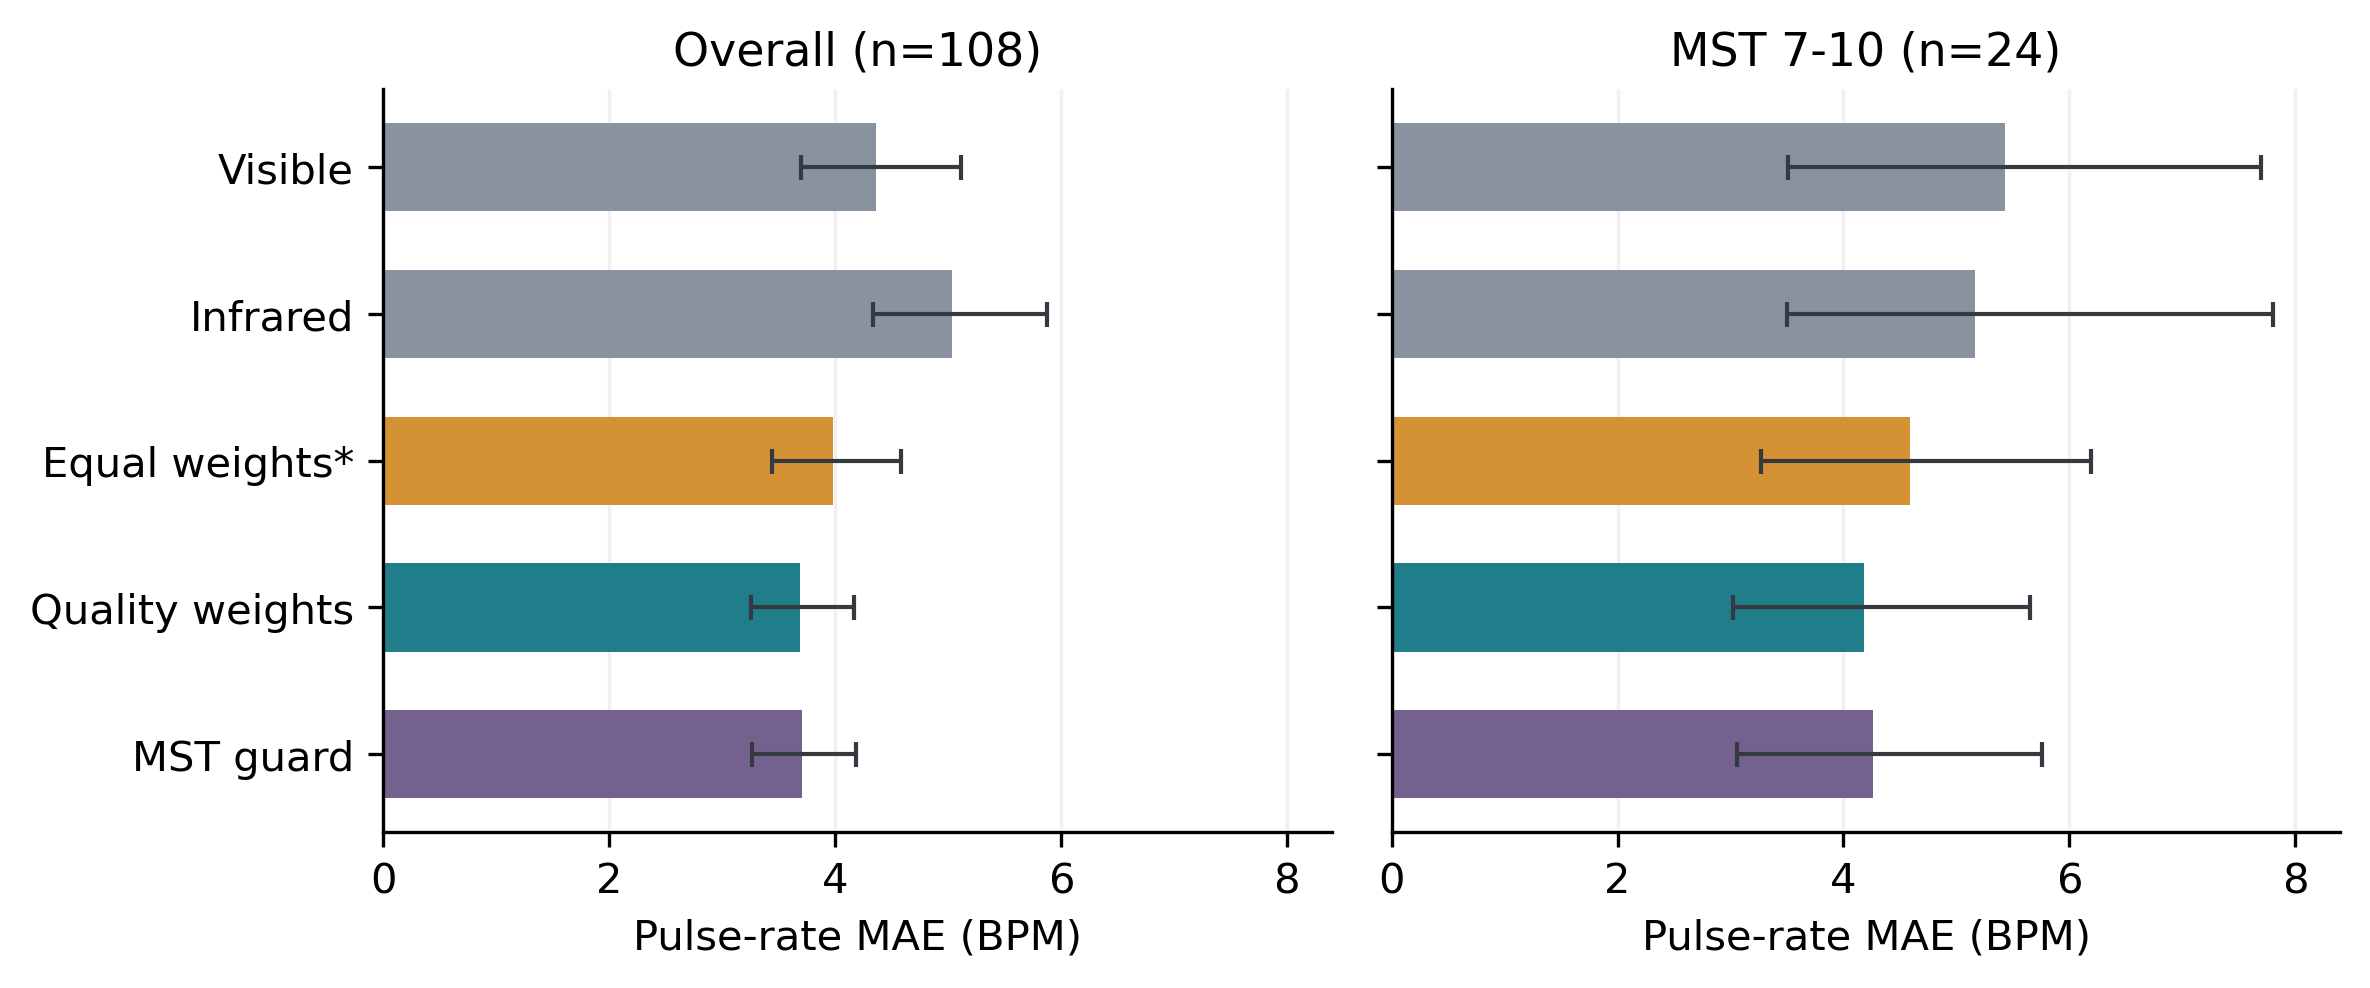
\includegraphics[width=\linewidth]{figures/fig_mendeley_quality_fusion.png}
\caption{Participant-balanced pulse-rate MAE with marginal 95\% bootstrap intervals. The equal-weight comparison was added post hoc; quality weighting improves overall error relative to equal weighting, while guarded MST correction does not establish additional benefit.}
\label{fig:mendeleyfusion}
\end{figure}

\subsection{VitalDB Context-Plus-PPG Frozen Holdout}
The expanded analysis used 55 development subjects to freeze the estimators and fixed blend, followed by one evaluation on 228 cases from 227 disjoint held-out subjects and 5{,}472 post-calibration windows. Table~\ref{tab:vitaldbpilot} separates the large gain over retaining the early calibration value from the stricter incremental PPG contrast. Calibration plus time/demographic context accounted for most of the improvement. The frozen fixed 50/50 blend reduced SBP MAE from $15.827$ to $15.375$~mmHg ($\Delta=-0.451$, 95\% CI $-0.781$ to $-0.121$) and DBP MAE from $9.189$ to $8.833$~mmHg ($\Delta=-0.357$, $-0.512$ to $-0.194$). It improved over context for $67.0\%$ of subjects for SBP and $70.5\%$ for DBP. For windows with $\geq10$~mmHg reference change, the incremental gains were $0.707$~mmHg SBP ($0.337$--$1.074$) and $0.501$~mmHg DBP ($0.274$--$0.726$). These results support a small incremental contribution of the PPG-augmented implementation within the VitalDB holdout, but absolute errors remain high and the test is retrospective and intraoperative rather than a prospective wearable validation.
\begin{table}[t]
\centering
\caption{VitalDB Context-Plus-PPG Frozen Holdout (227 Subjects)}
\label{tab:vitaldbpilot}
\scriptsize
\resizebox{\columnwidth}{!}{%
\begin{tabular}{lrrrr}
\toprule
Target & Retention & Context & Context+PPG & PPG$-$Context [95\% CI] \\
\midrule
SBP & 25.291 & 15.827 & 15.375 & $-0.451$ [$-0.781$, $-0.121$] \\
DBP & 13.098 & 9.189 & 8.833 & $-0.357$ [$-0.512$, $-0.194$] \\
\bottomrule
\end{tabular}}
\end{table}
\begin{figure}[t]
\centering
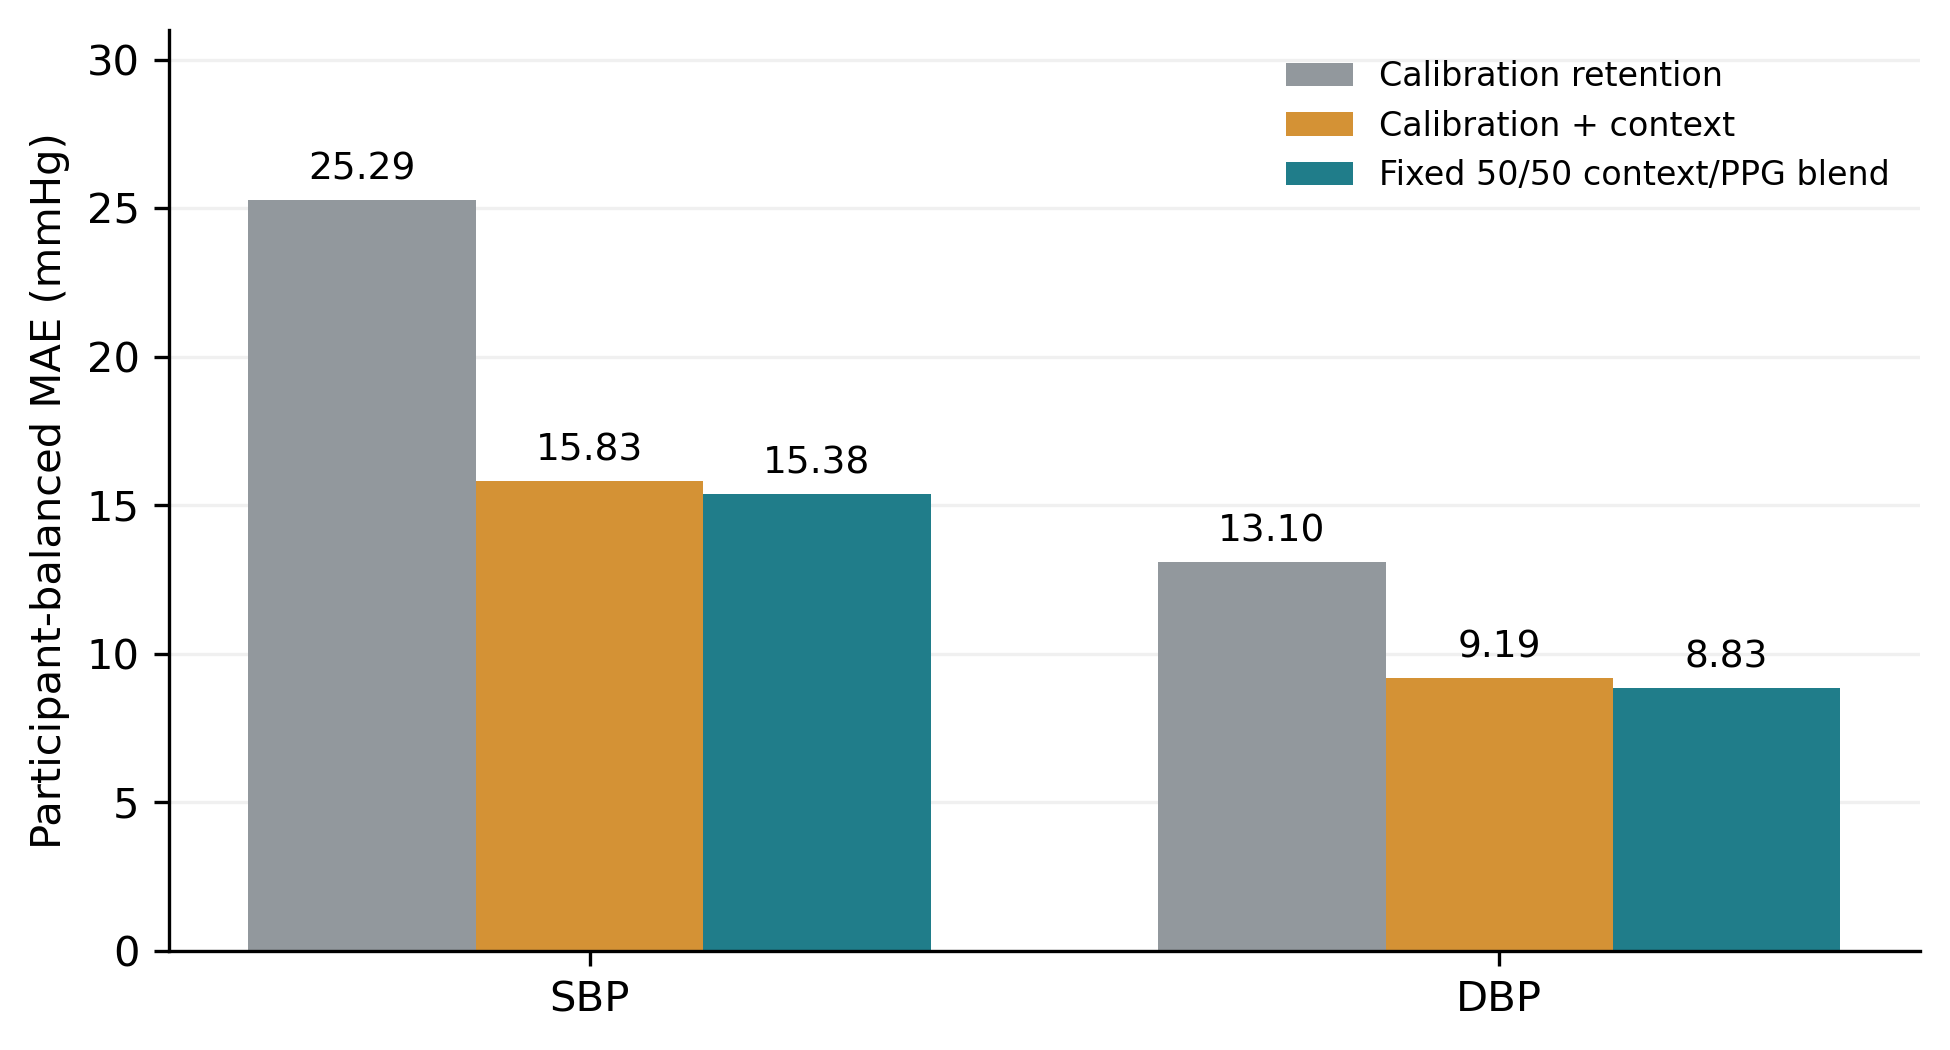
\includegraphics[width=\linewidth]{figures/fig_vitaldb_tracking.png}
\caption{VitalDB locked-holdout participant-balanced MAE. Calibration-plus-context explains most of the gain over retention; the frozen fixed context/PPG blend adds small CI-supported incremental improvements for both endpoints.}
\label{fig:vitaldbpilot}
\end{figure}
\subsection{State-of-the-Art Comparison}
\label{sec:sota}
Supplementary Table S9 compares representative cuffless-BP studies by dataset, participant separation, and calibration. Direct numerical ranking is inappropriate because populations, BP ranges, reference protocols, and calibration burdens differ; record-level leakage alone can materially change reported performance \cite{bpbenchmark2023}. The wearable-state MAE of $7.697$/$6.139$~mmHg is higher than the best calibrated reports and its DBP MAE is higher than the calibration-free result reported by \citet{calfree2023}. AuroraBP provides repeated internal validation with participant separation, whereas VitalDB evaluates a separately developed implementation in an intraoperative holdout. Neither analysis establishes wearable generalization or superiority over models evaluated under different protocols.
\section{Discussion}
\label{sec:discussion}
The primary AuroraBP comparison supports adding wearable-state context to the shared calibrated model, although posture and activity remain protocol annotations rather than independently estimated wearable states. The protocol-enriched arm achieves lower error but has greater dependence on acquisition metadata. Calibration dose materially affects that arm's performance. Because the common core already includes baseline BP, elapsed-time candidates, and a UCI prior, these results do not isolate PPG utility beyond a calibration-plus-context-only model on AuroraBP.

The independent studies answer different questions. The post-hoc equal-weight comparison supports quality-weighted pulse-rate fusion on the multi-wavelength dataset. VitalDB supports a small incremental BP contribution from a separately fitted context-plus-PPG implementation, combined with context through a fixed 50/50 blend. It does not test quality-dependent blending or transfer of AuroraBP-fitted parameters. The combined evidence supports calibrated tracking research but does not establish one universally generalizing architecture, an attractor-specific advantage, or clinical interchangeability. Pigmentation interventions remain secondary; small samples, possible indirect feature dependence, preclude fairness conclusions.

\textbf{Clinical accuracy boundary.} The method remains a research prototype for calibrated trend tracking. On the historical measurement-level standards analysis, SBP achieved BHS Grade~C and failed the reported AAMI/ISO Criterion~1 check because error SD was $9.654$~mmHg, above $8$~mmHg. VitalDB absolute MAE was also high ($15.375$/$8.833$~mmHg). These failures cannot be repaired by emphasizing relative improvements, rejecting difficult observations after seeing their errors, or treating a calibrated tracking model as a validated cuff-replacement device. Existing data can support tail-error diagnostics and prospectively defined repeat-measurement rules, but not a claim of clinical interchangeability.
\section{Limitations}
\label{sec:limitations}
\textbf{Validation and development.} AuroraBP is a controlled, single-site protocol with sessions shorter than one hour. Repeated participant-level cross-validation prevents direct participant overlap but cannot remove optimism from earlier choices made using this dataset. The independent Appel--Theart analysis concerns pulse extraction rather than BP, and VitalDB evaluates a separately developed retrospective intraoperative model rather than transfer of the AuroraBP model or prospective wearable performance.

\textbf{Calibration and context.} The primary result requires three initial cuff readings. The one-reading protocol-enriched model has higher MAE ($8.257$/$6.280$~mmHg), and a matching wearable-state dose analysis is unavailable. Posture and activity are recorded annotations rather than outputs of a deployed wearable classifier; phase, duration, and pressure-quality variables in the protocol-enriched arm may encode study structure.

\textbf{Pigmentation and fairness.} The repeated-CV cohort includes only 25 Fitzpatrick V--VI participants, and the historical fixed holdout includes six. The auxiliary-source pigmentation ranks are synthetic simulation inputs. The tested correction is one heuristic, and its null or adverse results establish neither equivalence nor the impossibility of a better intervention. The pulse-fusion study measures pulse-rate error, while VitalDB has no pigmentation labels; neither validates equitable BP performance.

\textbf{Inference, standards, and reproduction.} Holm adjustment covers only the two retrospectively designated primary endpoints; other analyses use exploratory marginal intervals. Participant-level summaries are used because repeated measurements are correlated. The DBP warning router has only $4.3\%$ recall and is not a safety mechanism. BHS and AAMI/ISO criteria were designed for absolute cuff-device validation and are included only as context. The rerun reproduces modeling and inference from hashed feature banks but does not repeat raw-waveform extraction. The matched ablation tests the combined nonlinear/attractor family and does not isolate any one descriptor.

\section{Conclusion}
\label{sec:conclusion}
This study provides retrospective evidence for context-augmented, session-calibrated BP tracking. Wearable context and standard PPG descriptors produced small incremental improvements, whereas the combined nonlinear/attractor family did not show a reliable additional benefit. Independent analyses supported quality-weighted pulse-rate fusion and a small PPG contribution within a separately developed VitalDB model. The results do not establish transfer of one model across datasets, equitable or prospective performance, standards compliance, or cuff replacement.
\section*{Code and Reproduction Availability}
The companion reproducibility package is publicly available on GitHub:
\begin{center}
\small\url{https://github.com/farouze/pc-avct-reproducibility}
\end{center}
It contains rerun and statistical scripts, the matched feature-family ablation, preserved V26 helper functions, pinned dependencies, SHA-256 input hashes, model-selection manifests, aggregate outputs, and sanitized development notebooks. Participant-level data, row predictions, and paired participant contrasts are excluded under the dataset access conditions and retained locally for audit. The versioned GitHub release is the software archive cited here; the dataset DOI below identifies data, not this implementation.
\section*{Data Availability}
AuroraBP is available from its provider upon application through the Zenodo record cited in \cite{aurorabpDataset} (DOI: 10.5281/zenodo.19099166) and acceptance of the Data Use Agreement. The authors are not permitted to redistribute AuroraBP participant-level data. BIDMC and MIMIC-II are available through PhysioNet, UCI Cuff-Less BP through the UCI Machine Learning Repository, the multi-wavelength data through Mendeley Data \cite{appel2025ppg}, and VitalDB through PhysioNet \cite{vitaldbDataset}. Access conditions and citations appear in Section~\ref{sec:datasets}. No directly identifying participant data are included in the manuscript or figures.
\section*{Ethics Statement}
This study is a secondary computational analysis of previously collected, deidentified human data. The authors recruited no participants, performed no intervention, had no participant contact, received no direct identifiers, and made no attempt to reidentify participants. Morgan State University's published IRB process states that submission is not required for research using deidentified data or publicly available datasets \cite{morganIRB2023}. Accordingly, this analysis did not require review by the Morgan State University Institutional Review Board, and no approval number was issued. The analysis followed the ethical principles of the Declaration of Helsinki and applicable local requirements. Ethics approvals and written informed-consent procedures for the original data collections are reported by the respective dataset providers and source publications \cite{aurorabp2022,aurorabpDataset,pimentel2017,appel2025ppg,lee2022vitaldb,vitaldbDataset}. No additional consent or consent for publication was required because the authors used only deidentified secondary data and report no identifiable participant information. This study was not a clinical trial.
\section*{Author Contributions}
Farouk Ganiyu Adewumi: conceptualization, methodology, software, validation, formal analysis, data curation, visualization, and writing of the original draft. Timothy Oladunni: conceptualization, methodology, supervision, and review and editing of the manuscript. Both authors approved this revised manuscript and the public code release.
\section*{Competing Interests}
The authors declare no competing financial or non-financial interests.
\section*{Funding}
This work was supported in part by Morgan State University's Office of Research and Graduate Programs.
\section*{Acknowledgment}
We thank the participants, investigators, and data stewards who made the secondary datasets used in this study available.
\bibliographystyle{plainnat}
\bibliography{references}

\ifdefined\INCLUDECOMBINEDSUPPLEMENT
\clearpage
\normalfont\normalsize
\appendices
\section{Supplementary Implementation Details}
\label{app:implementation}
\setcounter{table}{0}\renewcommand{\thetable}{S\arabic{table}}
\setcounter{figure}{0}\renewcommand{\thefigure}{S\arabic{figure}}
\subsection{Multi-Wavelength Pulse Processing}
For each device, visible and infrared pulse rates are estimated around the scheduled reference time using a window of up to 12~s, with at least 7.5~s and 150 samples required. Timestamps are converted to seconds, sorted, and deduplicated; signals are interpolated to a uniform grid using the median interval, with inferred sampling rate clipped to 20--500~Hz. A third-order 0.55--4~Hz Butterworth filter is applied forward and backward after detrending. Welch spectra use up to 8~s segments (at least 256 samples when available), with 50\% overlap. The dominant frequency is sought in 0.65--3.5~Hz; spectral concentration $c$ is the fraction of pulse-band power within 0.18~Hz of that peak.

An autocorrelation pulse estimate searches lags corresponding to 39--210~BPM. Let $a$ be the selected autocorrelation peak clipped to $[0,1]$, and $h_F,h_A$ the spectral and autocorrelation rates. When $|h_F-h_A|\leq15$~BPM, the channel estimate is $(c h_F+a h_A)/(c+a)$; otherwise the estimate with the larger reliability component is used. Channel quality is
\begin{align}
q&=\operatorname{clip}\!\left(\sqrt{ca}\,g,10^{-4},1\right),\\
g&=\begin{cases}1,&|h_F-h_A|\leq15,\\
e^{-|h_F-h_A|/30},&\text{otherwise.}\end{cases}
\end{align}
The tone-blind fusion estimate is $(q_Vh_V+q_Ih_I)/(q_V+q_I)$. The optional tone-dependent arm replaces the weights by $q_Ve^{-\alpha z}$ and $q_Ie^{\alpha z}$, with $z=\operatorname{clip}[(\mathrm{MST}-1)/9,0,1]$. Candidate $\alpha$ values are $\{0,\pm0.25,\pm0.5,\pm0.75,\pm1,\pm1.5,\pm2,\pm3\}$. Four participant folds within each outer training set score these fixed candidate rules. The selected nonzero exponent must improve mean fold MAE by at least 0.10~BPM and improve every inner fold; otherwise $\alpha=0$. The seed is 20260827, with repeat/fold offsets defined in the companion script. These methods estimate pulse rate, not BP.

\subsection{VitalDB Extraction and Model Selection}
Eligible cases have all three required tracks and a case duration of at least 1,800~s. Cases are deterministically shuffled with seed 20260827; positions 1--60 define development and 61--300 define the candidate holdout. The saved audit contains 55 development cases/subjects and 228 eligible holdout cases from 227 subjects, with no subject overlap. Eligibility and sampling are retrospective, and selecting windows across the completed record is not an online scheduling policy.

Candidate centers start no earlier than 120~s, proceed in 30-s increments, and require at least 900~s of usable overlapping record. PPG is retained at approximately 100~Hz. A 20-s window must contain at least 75\% of the expected samples and 85\% finite values; gaps are interpolated. Values are clipped to the median plus/minus eight robust SD estimates, detrended, and filtered with a third-order 0.5--8~Hz bandpass (upper cutoff limited by sampling rate). Pulse quality is spectral concentration multiplied by $\exp[-\min(\mathrm{interval\ CV},2)]$; windows below 0.04 are excluded. Pulse frequency search, spectral concentration, and beat-interval limits follow the companion extraction code. This quality filter is held fixed, but a no-quality-filter ablation is not reported.

Reference BP is the median of at least three plausible values within $\pm5$~s of the center. SBP must lie in 70--220~mmHg and DBP in 35--130~mmHg; local robust SD must not exceed 8 and 6~mmHg, respectively. Pulse pressure must lie in 20--130~mmHg. These reference-based exclusions do not use prediction errors but restrict the evaluated BP distribution. Cases require at least eight valid windows. The first three define median BP and feature anchors; up to 24 later windows are selected using evenly spaced indices over the valid future windows.

The context model uses anchor BP, $\log(1+\mathrm{elapsed\ seconds})$, age, sex, and preoperative hypertension (missing hypertension is coded as zero). The PPG model adds current and calibration-relative optical features listed by the \texttt{columns} function in the companion script. Candidate estimators comprise standardized ridge regression with 13 logarithmically spaced penalties from $10^{-3}$ to $10^3$ and three absolute-loss gradient-boosting configurations. Development-only five-fold participant validation selects estimators, followed by a fixed blend weight from $\{0,0.25,0.5,0.75,1\}$; a nonzero weight requires at least 0.10~mmHg improvement over context. Development selection is not independently nested across the estimator and blend choices, but holdout observations are excluded from both. Delta predictions are clipped at training-target 1st/99th percentiles.

Both endpoints selected ridge context models with penalty approximately 31.6228. The SBP PPG model uses absolute-loss boosting, learning rate 0.03, 15 leaves, regularization 5, 250 iterations, and minimum leaf size 20; the DBP PPG model uses ridge with penalty approximately 31.6228. Both selected a constant 0.5 PPG weight. The saved predictions satisfy this fixed-blend identity to numerical precision. Errors are averaged over all windows from all cases of a subject before subject bootstrap; the subject contributing two cases remains one bootstrap unit.

\subsection{Audit Scope and Reproduction Status}
The independent-dataset saved-result audit uses 10,000 participant bootstrap resamples with seed 20260910 for the pulse comparisons and verifies window uniqueness, case/subject counts, development/holdout separation, the fixed VitalDB blend, and the pulse-fusion equation. The AuroraBP analysis was separately rerun: the context arms and all three calibration doses were refitted across three repeats of five participant folds. The package records hashed feature inputs, software versions, selected features and gates, row-level outer-fold predictions, and paired participant contrasts. The historical subgroup model was also refitted. The rerun starts from feature banks; raw-waveform extraction is outside its scope.

\begin{table*}[t]
\centering
\caption{Interventions Tested and Not Adopted (Elimination Log)}
\label{tab:whatdidnotwork}
\begin{tabular}{p{4.6cm}p{2.4cm}p{7.8cm}}
\toprule
Intervention & Times tested & Outcome \\
\midrule
Absolute-error loss (vs.\ squared) & 3 & Never CI-supported: $+0.152$ [$-0.001$, 0.311] (51.8\% helped); $+0.102$ [$-0.028$, 0.240]; $+0.163$ [$-0.008$, 0.345] (exactly 50.0\% helped). \\
HCA feature augmentation & 2 & No CI-supported benefit: $-0.077$ [$-0.183$, 0.024]; $+0.043$ [$-0.026$, 0.115] (53.0\% helped). \\
Signal-level pigmentation (Beer--Lambert) correction & 2 & First variant increased error; the repeated-CV corrected channel changed MAE by $-0.007$ [$-0.042$, 0.029] SBP and $-0.030$ [$-0.062$, 0.003] DBP -- no established overall benefit (Section~\ref{sec:pcop}). \\
Demographic (Fitzpatrick-band) rebalancing / group gating & 5 & Consistently harmful: e.g., $-0.291$ [$-0.420,-0.170]$ mmHg SBP; widens between-band gap in every run (Section~\ref{sec:equity}). \\
Multi-window feature averaging & 1 & No measurable benefit; nominally worse (Section~\ref{sec:multiwindow}). \\
Nested gate/threshold search (early pipeline) & 1 & Higher error than a plainer reference baseline (8.253/8.183 vs.\ 8.109~mmHg SBP). \\
\midrule
\emph{Passed sanity check:} metadata-only permutation control & 1 & AUC $=0.492$ ($\approx$ chance) -- is consistent with chance under this permutation control; does not exclude other confounds. \\
\bottomrule
\end{tabular}
\end{table*}
\section{Historical Development and Auxiliary Analyses}
The following analyses preserve the development record. They are secondary or exploratory. The final subgroup subsection reports newly refitted estimates; development codes C0--C4 refer to the historical arms.
\subsection{Exploratory Endpoint-Specific Calibration and Warning Router}
\label{sec:v34}
Table~\ref{tab:v33primary} reports the historical post-primary endpoint analysis retained from the development record; it was not refitted in the V38 primary rerun. A nested, tightly clipped residual calibrator reduced SBP participant-level MAE from $7.611$ to $7.555$~mmHg, a paired improvement of $0.056$~mmHg (95\% CI $0.020$--$0.091$; $55.9\%$ of participants helped). The absolute gain is small, and tail behavior changed little (P90 absolute error $16.862 \to 16.820$~mmHg; P95 $22.184 \to 22.120$~mmHg). DBP candidate specialization did not improve inner-fold performance consistently, so the base prediction was retained at $5.784$~mmHg. This endpoint-specific policy is more conservative than adopting one post-processing rule for both targets.
\begin{table}[t]
\centering
\caption{Exploratory Endpoint-Specific Nested Analysis (653 Participants)}
\label{tab:v33primary}
\scriptsize
\resizebox{\columnwidth}{!}{%
\begin{tabular}{llrrr}
\toprule
Target & Arm & MAE & P90 AE & P95 AE \\
\midrule
SBP & Base & 7.611 & 16.862 & 22.184 \\
SBP & Clipped residual & \textbf{7.555} & 16.820 & 22.120 \\
DBP & Base & 5.784 & 12.043 & 15.630 \\
DBP & Selected policy & 5.784 & 12.043 & 15.630 \\
\midrule
\multicolumn{5}{l}{\footnotesize SBP paired gain: 0.056 mmHg [0.020, 0.091]; DBP gain: 0.000.} \\
\bottomrule
\end{tabular}
}
\end{table}
The exploratory DBP router was therefore frozen as warning-only. Extreme DBP change prevalence was $20.5\%$ (95\% CI $19.1$--$21.9\%$). The router achieved ROC AUC $0.794$ ($0.778$--$0.809$), average precision $0.517$ ($0.483$--$0.555$), and Brier score $0.130$ ($0.122$--$0.137$). At the nested operating threshold, warning precision was $0.773$ ($0.695$--$0.854$), but recall was only $0.043$ ($0.035$--$0.052$) and the warning rate was $1.1\%$ ($0.9$--$1.4\%$). The router is thus a rare high-precision flag at the evaluated threshold; it is not a screen for most extreme changes, does not reduce reported DBP MAE, and must not be interpreted as a clinical safety mechanism.
\subsection{Historical Duplicate-Reading Noise Diagnostic}
Table~\ref{tab:noisefloor} retains a historical duplicate-reading diagnostic, not a universal achievable-error bound. Estimating per-reading noise as $\sigma_{P-S}/\sqrt{2}$ assumes independent, equal-variance observer errors. The supplied code distinguishes a stored average of two readings from a single-reading target and propagates target and anchor errors for a legacy two-time-point difference. Its $1.754$/$2.412$~mmHg Gaussian absolute-noise estimates and $2.6\%$/$9.2\%$ variance ratios therefore must not be treated as validated floors for the primary three-reading anchor. Shared observer error, physiological change during measurement, and the actual target-averaging rule can change the estimates. A primary-endpoint noise calculation would require those components and their covariances; subtracting a putative floor from model MAE does not measure recoverable physiological error.
\begin{table}[t]
\centering
\caption{Historical Duplicate-Reading Diagnostic (8{,}918/8{,}916 SBP/DBP pairs)}
\label{tab:noisefloor}
\begin{tabular}{lrr}
\toprule
Quantity (mmHg) & SBP & DBP \\
\midrule
$\sigma$(primary $-$ secondary reading) & 3.108 & 4.275 \\
$\sigma_{\mathrm{cuff}}$ (per-reading noise) & 2.198 & 3.023 \\
Legacy Gaussian absolute-noise estimate & 1.754 & 2.412 \\
Observed SD of $\Delta$ & 13.70 & 9.98 \\
Legacy noise/observed variance ratio & 2.6\% & 9.2\% \\
Residual SD under legacy assumptions & 13.52 & 9.51 \\
Early reference model MAE & 8.11 & -- \\
\bottomrule
\end{tabular}
\end{table}
\subsection{Recalibration Cadence}
The historical code evaluated nominal recalibration intervals of 1, 3, 6, 12, and 24~h, with nearly identical MAE ($8.593$--$8.594$~mmHg SBP; $6.020$--$6.022$~mmHg DBP). Those labels do not establish distinct effective recalibration schedules in the analyzed short laboratory sessions. The stored comparison lacks an event-count and elapsed-time audit sufficient to interpret a cadence effect. We therefore withdraw the inference that cadence beyond one hour is immaterial and make no recommendation about recalibration frequency from this analysis.
\subsection{Multi-Window Feature Averaging}
\label{sec:multiwindow}
Averaging attractor features over multiple 10~s windows per recording (up to 3 available) was hypothesized to reduce measurement noise (Table~\ref{tab:multiwindow} shows within/between SD ratios up to approximately 0.45). It did not help: holdout MAE with multi-window averaging ($6.393$/$4.828$~mmHg SBP/DBP) was statistically indistinguishable from, and nominally slightly worse than, a matched single-window configuration ($6.346$/$4.803$~mmHg), both close to the legacy single-window baseline ($6.315$/$4.789$~mmHg). We report this as a negative result (Table~\ref{tab:whatdidnotwork}).
\begin{table}[t]
\centering
\caption{Historical Within- and Between-Recording Feature SD}
\label{tab:multiwindow}
\begin{tabular}{lrrr}
\toprule
Feature & Within SD & Between SD & SD ratio \\
\midrule
$\sigma_m$ & 0.0046 & 0.0102 & 0.449 \\
CSI & 0.0043 & 0.0138 & 0.311 \\
Recurrence rate & 0.0040 & 0.0130 & 0.305 \\
Kurtosis & 0.0902 & 0.3086 & 0.292 \\
RQA entropy & 0.0734 & 0.2520 & 0.291 \\
Skewness & 0.0386 & 0.1389 & 0.278 \\
Sample entropy & 0.0133 & 0.0527 & 0.252 \\
Determinism & 0.0114 & 0.0475 & 0.240 \\
Spectral entropy & 0.0092 & 0.0488 & 0.189 \\
Permutation entropy & 0.0028 & 0.0190 & 0.150 \\
\bottomrule
\end{tabular}
\end{table}

\subsection{Historical Fixed-Split Session-Anchored Ladder}
\label{sec:v23}
During earlier development, the model-development ladder was evaluated on a fixed 501/168 participant split. Table~\ref{tab:v23} preserves that analysis for transparency: C4 reduced MAE from $8.856$/$6.582$ to $7.147$/$5.579$~mmHg. Because the same 168 participants were examined across successive ablations, these values are historical development evidence and are not the paper's primary validation result. The corresponding repeated participant-validation estimates in Table~\ref{tab:v26primary} are modestly worse ($7.523$/$5.743$~mmHg for protocol-enriched context), consistent with mild optimism from the fixed split rather than a collapse of the effect.
\begin{table}[t]
\centering
\caption{Historical Fixed-Split Session-Anchored Ladder (168 Evaluation Participants)}
\label{tab:v23}
\resizebox{\columnwidth}{!}{%
\begin{tabular}{lrrr}
\toprule
Arm & SBP MAE [95\% CI] & DBP MAE [95\% CI] \\
\midrule
Calibration retention & 8.856 & 6.582 \\
C0 legacy (squared) & 7.956 [7.424, 8.501] & 6.120 [5.641, 6.647] \\
C1 absolute loss & 7.793 [7.270, 8.316] & 6.014 [5.513, 6.546] \\
C2 +context & 7.156 [6.740, 7.618] & 5.651 [5.186, 6.146] \\
C3 +context+HCA & 7.113 [6.703, 7.550] & 5.636 [5.178, 6.126] \\
\textbf{C4 +context (squared)} & \textbf{7.147 [6.736, 7.593]} & \textbf{5.579 [5.174, 6.004]} \\
\midrule
Reduction, calib.\ $\rightarrow$ C4 & \textbf{1.709 (19.3\%)} & \textbf{1.003 (15.2\%)} \\
\bottomrule
\end{tabular}
}
\end{table}
\begin{figure}[t]
\centering
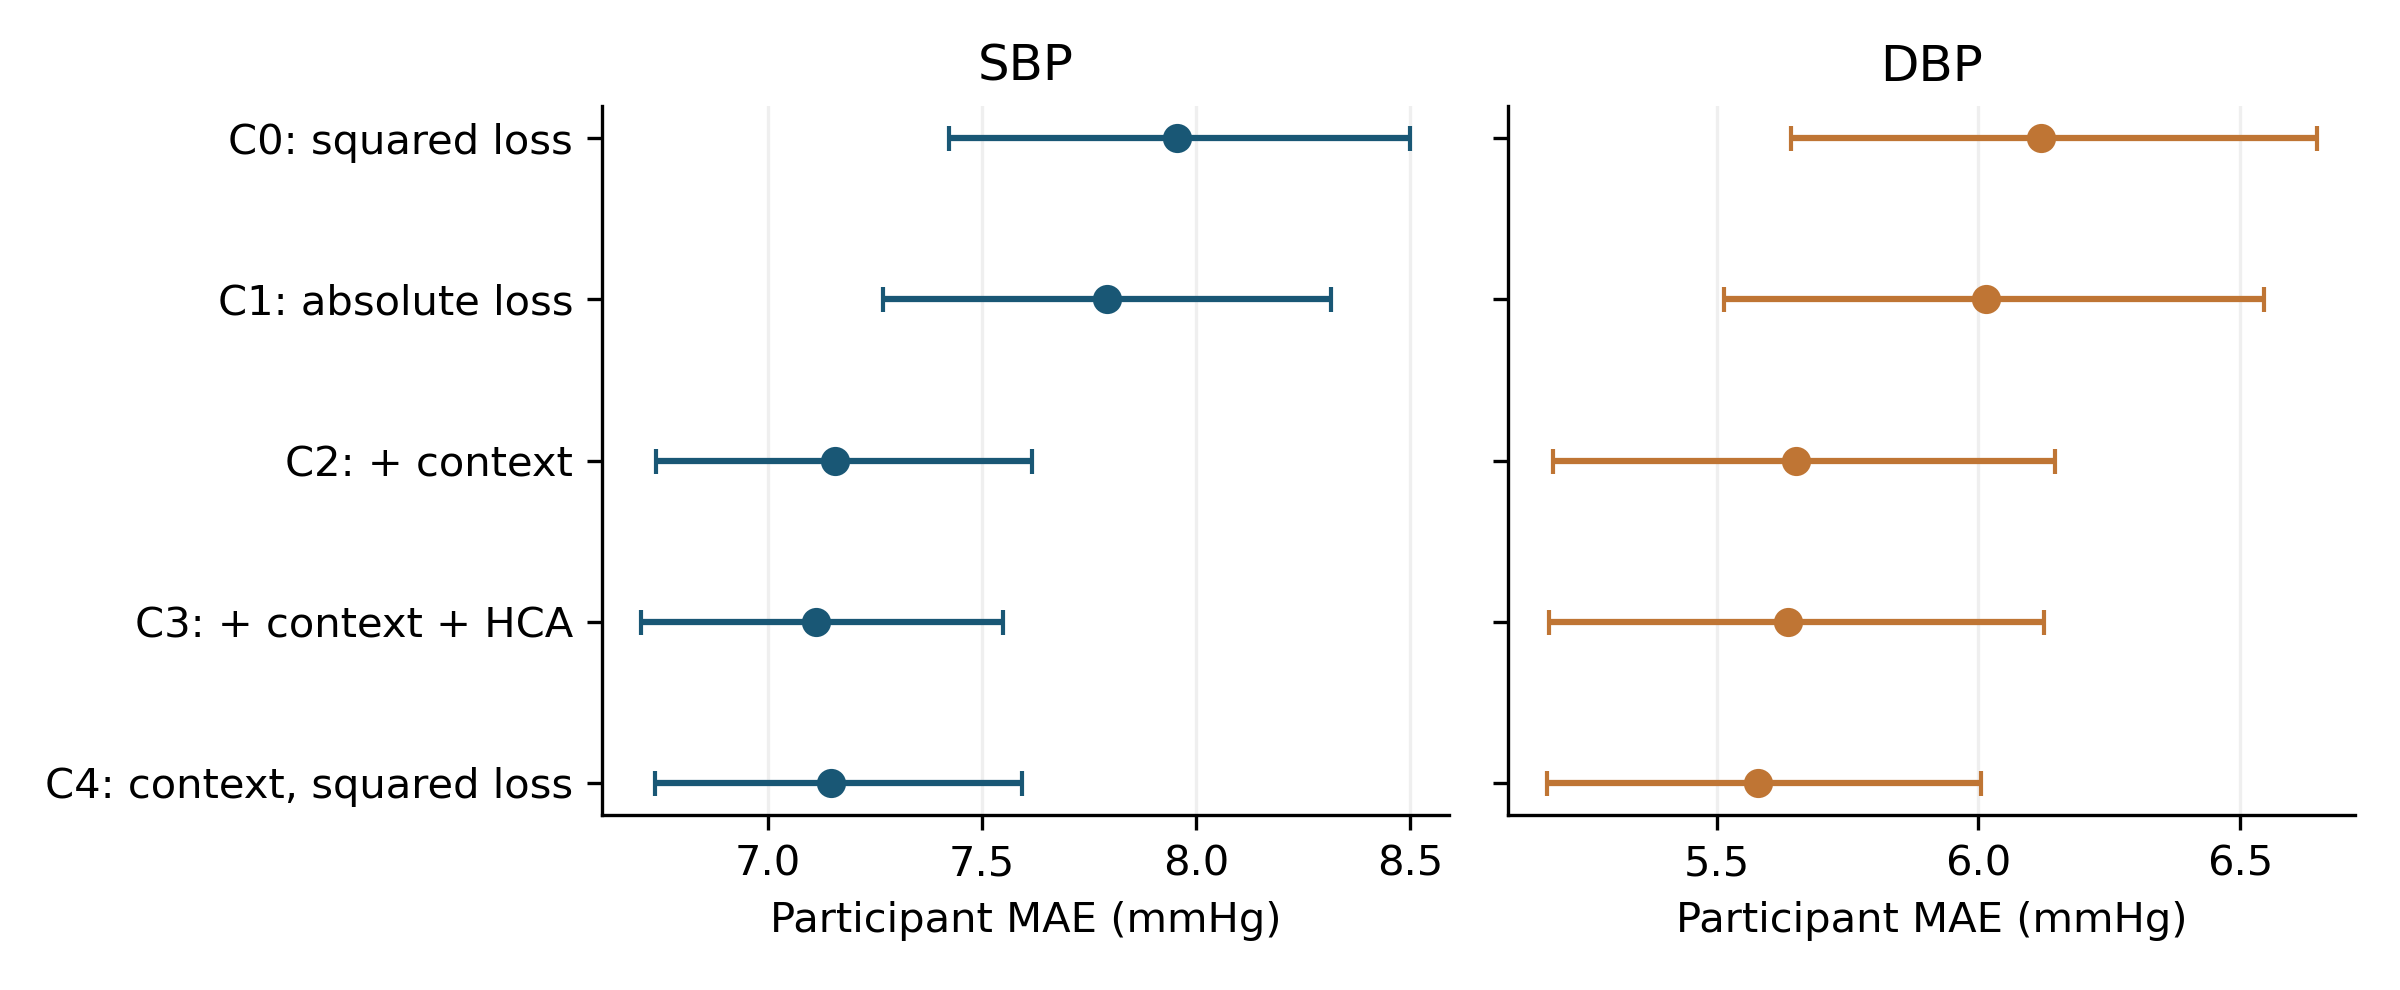
\includegraphics[width=\linewidth]{figures/fig_ladder.png}
\caption{Historical fixed-split session-anchored ladder with 95\% participant-bootstrap CIs. This figure documents model development; Table~\ref{tab:v26primary} provides the primary repeated participant-validation result.}
\label{fig:ladder}
\end{figure}
\subsection{Calibration-Row Leakage Audit}
\label{sec:leakage-results}
Table~\ref{tab:leakage} reports all four checks from Section~\ref{sec:leakage}. Check A shows calibration-flagged rows are smaller in mean $|\Delta|$ than unflagged rows ($6.774$ vs.\ $9.902$~mmHg SBP, development set) but not trivially near-zero, and the fraction of rows within 1~mmHg is nearly identical between flagged and unflagged rows ($9.8\%$ vs.\ $8.6\%$). The decisive Check D -- flag removed from features, flagged rows excluded from both fit and scoring -- yields a context gain of $+0.614$~mmHg SBP $[0.346, 0.889]$ and $+0.513$~mmHg DBP $[0.268, 0.743]$, both CI-supported and close to the unaudited historical figures. Leave-one-out attribution (Figure~\ref{fig:loo}) shows larger predictive contributions from recording duration and post-exercise activity, not the calibration flag (LOO damage for the flag: $0.0000$ SBP / $0.0027$ DBP).
\begin{table}[t]
\centering
\caption{Calibration-Row Leakage Audit (168 holdout participants)}
\label{tab:leakage}
\scriptsize
\resizebox{\columnwidth}{!}{%
\begin{tabular}{p{2.3cm}p{2.0cm}p{2.0cm}c}
\toprule
Check & SBP gain [CI] & DBP gain [CI] & Verdict \\
\midrule
B (flagged excl.) & 0.741 [0.440, 1.062] & 0.606 [0.372, 0.854] & Supp. \\
C (flag dropped) & 0.809 [0.501, 1.122] & 0.538 [0.309, 0.770] & Supp. \\
\textbf{D (strict)} & \textbf{0.614 [0.346, 0.889]} & \textbf{0.513 [0.268, 0.743]} & \textbf{Supp.} \\
\bottomrule
\end{tabular}
}
\end{table}
\begin{figure}[t]
\centering
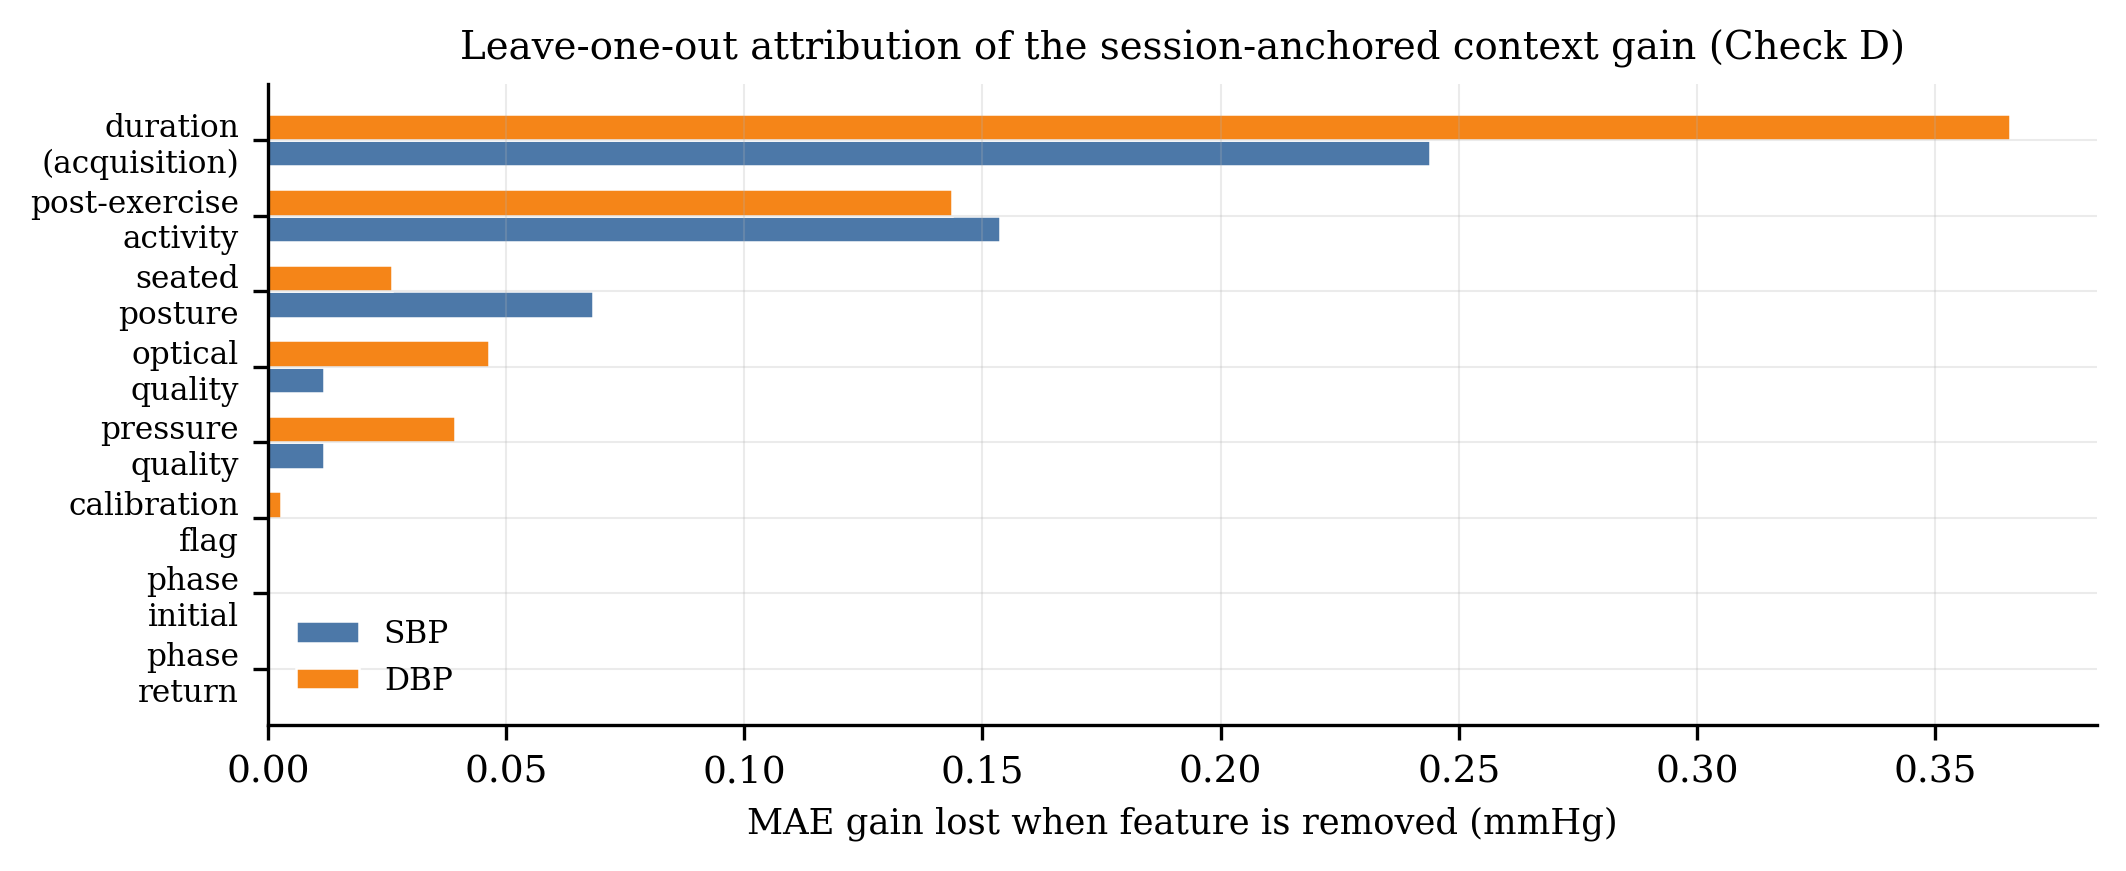
\includegraphics[width=\linewidth]{figures/fig_loo_context.png}
\caption{Leave-one-out attribution of the session-anchored context gain (Check D). The largest contributor is recording duration -- an acquisition property, not a purely physiological one -- followed by post-exercise activity.}
\label{fig:loo}
\end{figure}
One honest qualification: the single largest contributor to the context gain is recording \emph{duration} ($0.244$~mmHg SBP / $0.366$~mmHg DBP of leave-one-out damage), which is an acquisition property (likely proxying protocol step or signal stability) rather than a purely physiological state variable. ``Context = posture and activity'' is only partly right; post-exercise activity ($0.154$/$0.144$~mmHg) is the clearest genuinely physiological contributor, with posture third.

\subsection{Clinical Standards Context}
Table~\ref{tab:bhsaami} reports BHS grading and AAMI/ISO~81060-2 Criterion~1 for the C4 session-anchored model. The model improves cumulative within-5/10/15~mmHg percentages over both calibration retention and the legacy baseline for both SBP and DBP, and reaches BHS Grade~B for DBP (Grade~C for SBP); it passes AAMI Criterion~1 for DBP (mean error $0.645$, SD $7.992 \leq 8$~mmHg) but not for SBP (SD $9.654 > 8$~mmHg). \textbf{We report both gradings as indicative context, not a validation claim}: BHS and AAMI/ISO were written for cuff devices measuring absolute BP against an independent reference, and this model is calibrated per participant.
\begin{table}[t]
\centering
\caption{BHS Grading and AAMI/ISO 81060-2 Criterion 1 (Session-Anchored C4 Model, Measurement-Level)}
\label{tab:bhsaami}
\scriptsize
\resizebox{\columnwidth}{!}{%
\begin{tabular}{lccccc}
\toprule
Target/Arm & $\leq$5mm & $\leq$10mm & $\leq$15mm & Grade & AAMI-1 \\
\midrule
SBP calibration & 45.9\% & 72.3\% & 83.9\% & D & Fail \\
SBP baseline (C0) & 45.8\% & 73.8\% & 86.6\% & C & Fail \\
SBP model (C4) & 48.0\% & 75.1\% & 89.7\% & C & Fail \\
DBP calibration & 56.0\% & 82.9\% & 92.2\% & B & Fail \\
DBP baseline (C0) & 56.0\% & 83.1\% & 93.6\% & B & Fail \\
DBP model (C4) & 58.7\% & 85.6\% & 94.9\% & B & \textbf{Pass} \\
\bottomrule
\end{tabular}
}
\end{table}
\subsection{What Did Not Work}
\label{sec:whatdidnotwork}
Table~\ref{tab:whatdidnotwork} summarizes every intervention tested and rejected in this study, alongside one passed sanity check. We regard this table as carrying as much evidentiary weight as Table~\ref{tab:v23}: a result that survives repeated, adversarially-minded attempts to break it is more credible than one presented without them.


\subsection{Refitted Fixed-Estimator and Primary-Cohort Subgroups}
The historical prior-anchored estimator was refitted under the recorded environment, and Table~\ref{tab:fixedfst} reports its newly generated predictions. These estimates supersede the earlier rounded subgroup values; they do not assert bitwise recovery of the original run. The companion change record retains the old-value comparison. The same estimator is applied within each analysis before predictions are grouped by Fitzpatrick band. The primary wearable-state summary uses the independently regenerated repeated-CV predictions, not the historical fixed split.
\begin{table}[t]
\centering
\caption{Regenerated Participant MAE by Fitzpatrick Band}
\label{tab:fixedfst}
\scriptsize
\resizebox{\columnwidth}{!}{%
\begin{tabular}{lllrr}
\toprule
Analysis & Target & Band ($n$) & MAE & 95\% CI \\
\midrule
Prior refit & SBP & I--II (133) & 5.837 & [5.513, 6.178] \\
Prior refit & SBP & III--IV (29) & 5.568 & [4.703, 6.549] \\
Prior refit & SBP & V--VI (6) & 5.341 & [3.847, 6.841] \\
Prior refit & DBP & I--II (133) & 4.439 & [4.118, 4.795] \\
Prior refit & DBP & III--IV (29) & 4.781 & [3.674, 6.370] \\
Prior refit & DBP & V--VI (6) & 4.020 & [2.931, 5.197] \\
\midrule
Primary CV & DBP & I--II (516) & 6.078 & [5.805, 6.362] \\
Primary CV & DBP & III--IV (112) & 6.435 & [5.862, 7.045] \\
Primary CV & DBP & V--VI (25) & 6.053 & [5.065, 7.122] \\
Primary CV & SBP & I--II (516) & 7.680 & [7.355, 8.022] \\
Primary CV & SBP & III--IV (112) & 7.786 & [7.050, 8.610] \\
Primary CV & SBP & V--VI (25) & 7.646 & [6.052, 9.471] \\
\bottomrule
\end{tabular}}
\end{table}
These are exploratory marginal intervals. Differences in sample size, anchoring, and validation design prevent direct comparison between the two analysis blocks. In particular, the small V--VI samples do not establish parity or equivalence, irrespective of the ordering of the point estimates.
\fi
\end{document}
